\documentclass{beamer}
\usepackage{amsmath,amssymb,amsthm,graphicx}
\usepackage{color}
\usetheme{Gerrish}
\usepackage[mathcal]{euscript}   % for script letters
\usepackage{array}
\usepackage{bm}
\usepackage{wrapfig}
\usepackage{multirow}

\setbeamertemplate{navigation symbols}{}
\setbeamertemplate{outlinem}{}

\newcommand{\z}{\textbf{z}} 
\newcommand{\W}{\textbf{W}}
\newcommand{\mv}{\tilde{m}} 
\newcommand{\vv}[0]{\tilde{V}}
\newcommand{\w}{\textbf{w}}
\newcommand{\vphi}{\phi}
\newcommand{\bv}{\tilde{\beta}}
\newcommand{\bb}{\beta}
\newcommand{\lv}{\tilde{l}}
\newcommand{\vlv}{\sigma^2_{l}}
\newcommand{\vd}{\sigma^2_{d}}
\newcommand{\vbv}{\sigma^2}
\newcommand{\stdnorm}[1]{\mathcal{N}\left(#1\right)}


\newcommand{\tr}[0]{\mbox{Tr}}
\newcommand{\expectq}[1]{\mathbb{E}_q\left[#1\right]}
\newcommand{\expectqnoarg}[0]{\mathbb{E}_q}
\newcommand{\defn}[0]{:=}
\newcommand{\partl}[2]{\frac{\partial #1}{\partial #2}}


\title{Predicting legislative votes with text}
 \subtitle{} \date{1 June 2011} \author{Sean Gerrish and David Blei \\
   Princeton University Computer Science}

\begin{document}
\frame{\titlepage}

\section{Introduction}

\section{The problem}

%% \frame {
%%   Thanks,
%%   \newline
%%   \begin{center}
%%   \includegraphics[width=0.6\textwidth]{../figures/ps_logo2.png} \newline
%%   \includegraphics[width=0.4\textwidth]{../figures/nsf1.jpg}
%%   \end{center}
%% }

\frame {
 \frametitle{Predicting Legislative Votes}
  \hspace{155pt}
  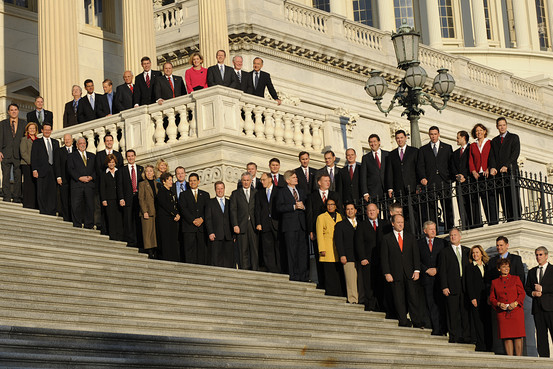
\includegraphics[width=0.34\textwidth]{figs/newcongress_photo_G_20090105182921.jpg}
  \[
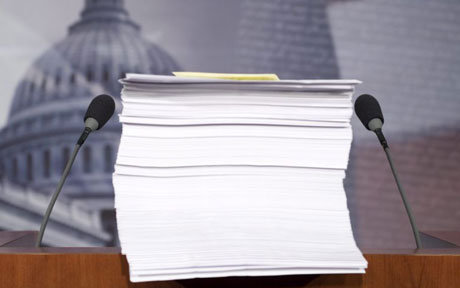
\includegraphics[width=0.34\textwidth,bb=30 110 450 230]{figs/health-bill.jpg}
  \left[
   \begin{array}{cccccccc}
     \textcolor{black}{Y} & & & \textcolor{black}{N} & \textcolor{black}{Y} &  & & \textcolor{black}{Y} \\
     & & & &                    &  & \textcolor{black}{N}  & \\
     & & \textcolor{black}{Y} & & &  & & \\
     \textcolor{black}{Y} & & & &                    & \textcolor{black}{N} &        & \textcolor{black}{N} \\
     \textcolor{black}{N} & \textcolor{black}{N} & & & \textcolor{black}{Y} &  & & \textcolor{black}{Y} \\
     & & & &                    &  &  & \textcolor{black}{N} \\
     & & & & \textcolor{white}{Y} &  & \textcolor{white}{Y} & \\
     \textcolor{white}{Y} & \textcolor{white}{Y} & & &                    &  & & \textcolor{white}{N} \\
     & & \textcolor{white}{N} & \textcolor{white}{Y} &                    & \textcolor{white}{Y} & &  \\
    \textcolor{white}{Y} & \textcolor{white}{N} & & & & & \textcolor{white}{Y} & \\
   \end{array}
   \right]
\]
\tiny 
Images credit Susan Walsh (Associated Press) and EPA
\normalsize
}

\frame {
 \frametitle{Predicting Legislative Votes}
  \hspace{155pt}
  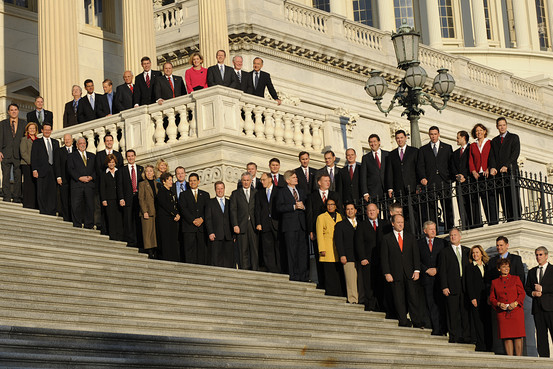
\includegraphics[width=0.34\textwidth]{figs/newcongress_photo_G_20090105182921.jpg}
  \[
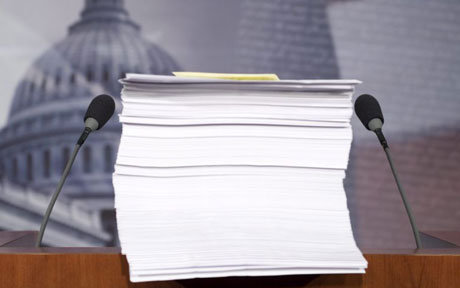
\includegraphics[width=0.34\textwidth,bb=30 110 450 230]{figs/health-bill.jpg}
  \left[
   \begin{array}{cccccccc}
     \textcolor{black}{Y} & & & \textcolor{black}{N} & \textcolor{black}{Y} &  & & \textcolor{black}{Y} \\
     & & & &                    &  & \textcolor{black}{N}  & \\
     & & \textcolor{black}{Y} & & &  & & \\
     \textcolor{black}{Y} & & & &                    & \textcolor{black}{N} &        & \textcolor{black}{N} \\
     \textcolor{black}{N} & \textcolor{black}{N} & & & \textcolor{black}{Y} &  & & \textcolor{black}{Y} \\
     & & & &                    &  &  & \textcolor{black}{N} \\
     & & & & \textcolor{black}{Y} &  & \textcolor{black}{Y} & \\
     \textcolor{white}{Y} & \textcolor{white}{Y} & & &                    &  & & \textcolor{white}{N} \\
     & & \textcolor{white}{N} & \textcolor{white}{Y} &                    & \textcolor{white}{Y} & &  \\
    \textcolor{white}{Y} & \textcolor{white}{N} & & & & & \textcolor{white}{Y} & \\
   \end{array}
   \right]
\]
\tiny 
Images credit Susan Walsh (Associated Press) and EPA
\normalsize
}

\frame {
 \frametitle{Predicting Legislative Votes}
  \hspace{155pt}
  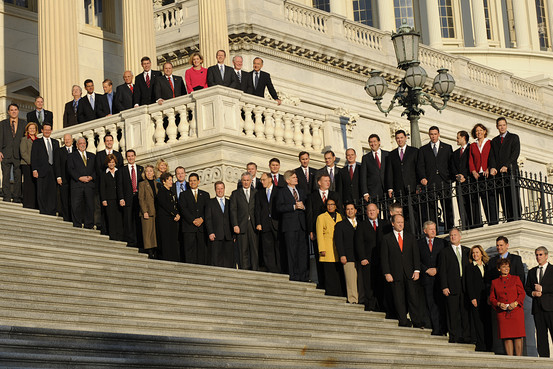
\includegraphics[width=0.34\textwidth]{figs/newcongress_photo_G_20090105182921.jpg}
  \[
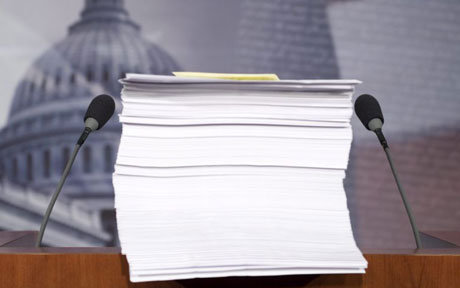
\includegraphics[width=0.34\textwidth,bb=30 110 450 230]{figs/health-bill.jpg}
  \left[
   \begin{array}{cccccccc}
     \textcolor{black}{Y} & & & \textcolor{black}{N} & \textcolor{black}{Y} &  & & \textcolor{black}{Y} \\
     & & & &                    &  & \textcolor{black}{N}  & \\
     & & \textcolor{black}{Y} & & &  & & \\
     \textcolor{black}{Y} & & & &                    & \textcolor{black}{N} &        & \textcolor{black}{N} \\
     \textcolor{black}{N} & \textcolor{black}{N} & & & \textcolor{black}{Y} &  & & \textcolor{black}{Y} \\
     & & & &                    &  &  & \textcolor{black}{N} \\
     & & & & \textcolor{black}{Y} &  & \textcolor{black}{Y} & \\
     \textcolor{black}{Y} & \textcolor{black}{Y} & & &                    &  & & \textcolor{black}{N} \\
     & & \textcolor{white}{N} & \textcolor{white}{Y} &                    & \textcolor{white}{Y} & &  \\
    \textcolor{white}{Y} & \textcolor{white}{N} & & & & & \textcolor{white}{Y} & \\
   \end{array}
   \right]
\]
\tiny 
Images credit Susan Walsh (Associated Press) and EPA
\normalsize
}

\frame {
 \frametitle{Predicting Legislative Votes}
  \hspace{155pt}
  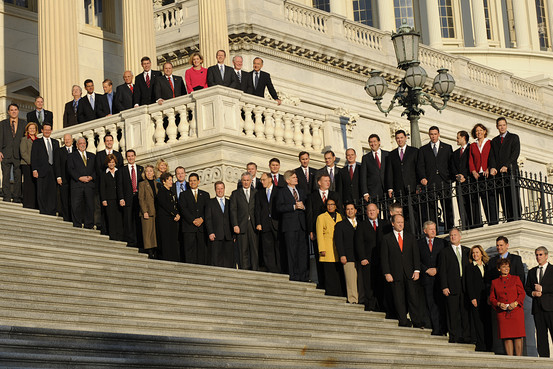
\includegraphics[width=0.34\textwidth]{figs/newcongress_photo_G_20090105182921.jpg}
  \[
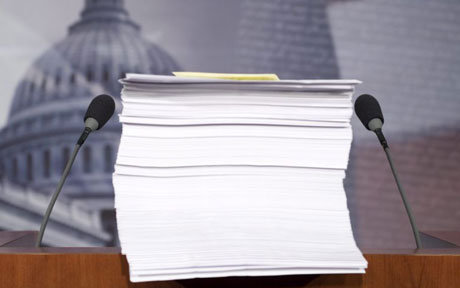
\includegraphics[width=0.34\textwidth,bb=30 110 450 230]{figs/health-bill.jpg}
  \left[
   \begin{array}{cccccccc}
     \textcolor{black}{Y} & & & \textcolor{black}{N} & \textcolor{black}{Y} &  & & \textcolor{black}{Y} \\
     & & & &                    &  & \textcolor{black}{N}  & \\
     & & \textcolor{black}{Y} & & &  & & \\
     \textcolor{black}{Y} & & & &                    & \textcolor{black}{N} &        & \textcolor{black}{N} \\
     \textcolor{black}{N} & \textcolor{black}{N} & & & \textcolor{black}{Y} &  & & \textcolor{black}{Y} \\
     & & & &                    &  &  & \textcolor{black}{N} \\
     & & & & \textcolor{black}{Y} &  & \textcolor{black}{Y} & \\
     \textcolor{black}{Y} & \textcolor{black}{Y} & & &                    &  & & \textcolor{black}{N} \\
     & & \textcolor{black}{N} & \textcolor{black}{Y} &                    & \textcolor{black}{Y} & &  \\
    \textcolor{white}{Y} & \textcolor{white}{N} & & & & & \textcolor{white}{Y} & \\
   \end{array}
   \right]
\]
\tiny 
Images credit Susan Walsh (Associated Press) and EPA
\normalsize
}

\frame {
 \frametitle{Predicting Legislative Votes}

  \hspace{155pt}
  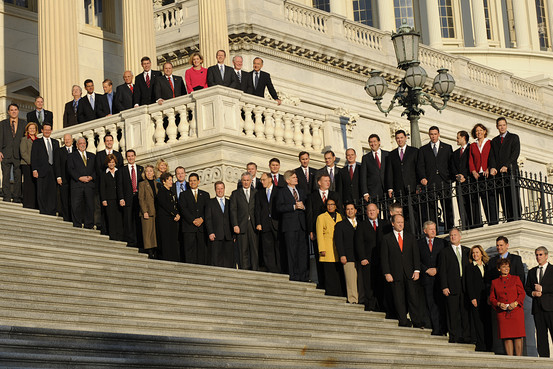
\includegraphics[width=0.34\textwidth]{figs/newcongress_photo_G_20090105182921.jpg}
  \[
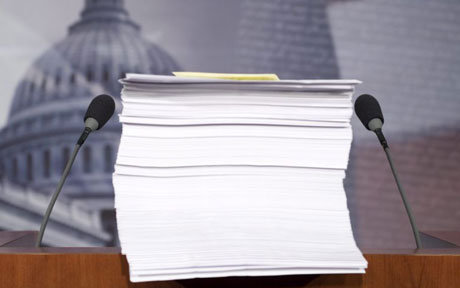
\includegraphics[width=0.34\textwidth,bb=30 110 450 230]{figs/health-bill.jpg}
  \left[
   \begin{array}{cccccccc}
     \textcolor{black}{Y} & & & \textcolor{black}{N} & \textcolor{black}{Y} &  & & \textcolor{black}{Y} \\
     & & & &                    &  & \textcolor{black}{N}  & \\
     & & \textcolor{black}{Y} & & &  & & \\
     \textcolor{black}{Y} & & & &                    & \textcolor{black}{N} &        & \textcolor{black}{N} \\
     \textcolor{black}{N} & \textcolor{black}{N} & & & \textcolor{black}{Y} &  & & \textcolor{black}{Y} \\
     & & & &                    &  &  & \textcolor{black}{N} \\
     & & & & \textcolor{black}{Y} &  & \textcolor{black}{Y} & \\
     \textcolor{black}{Y} & \textcolor{black}{Y} & & &                    &  & & \textcolor{black}{N} \\
     & & \textcolor{black}{N} & \textcolor{black}{Y} &                    & \textcolor{black}{Y} & &  \\
     \textcolor{blue}{?} & \textcolor{blue}{?} & & & & & \textcolor{blue}{?} & \\
   \end{array}
   \right]
\]
\tiny
Images credit Susan Walsh (Associated Press) and EPA
\normalsize
}

% \frame{
%   \frametitle{Goal of this work}

%   We have two goals: \\
%   \begin{enumerate}
%     \item to predict votes on legislative text \\
%     \item to understand the issues driving these votes \\
%   \end{enumerate}

%   To achieve these goals, we will combine ideas from political science with machine learning: \\
%   \begin{itemize}
%     \item ideal point models \\
%     \item text regression and topic models \\
%   \end{itemize}
% }

\frame{
  \frametitle{Organization}
  Introduce models \\

  \begin{itemize}
  \item Overview of a model to represent votes \\
  \item Link from documents text to voting model parameters \\
  \item Inference on these models \\
  \end{itemize}

  Experimental results \\
  \begin{itemize}
  \item Predictive performance \\
  \item Text and political sentiment \\
  \item Next steps and conclusions \\
  \end{itemize}

}


% \frame{
%   \frametitle{A model of voting patterns}
%   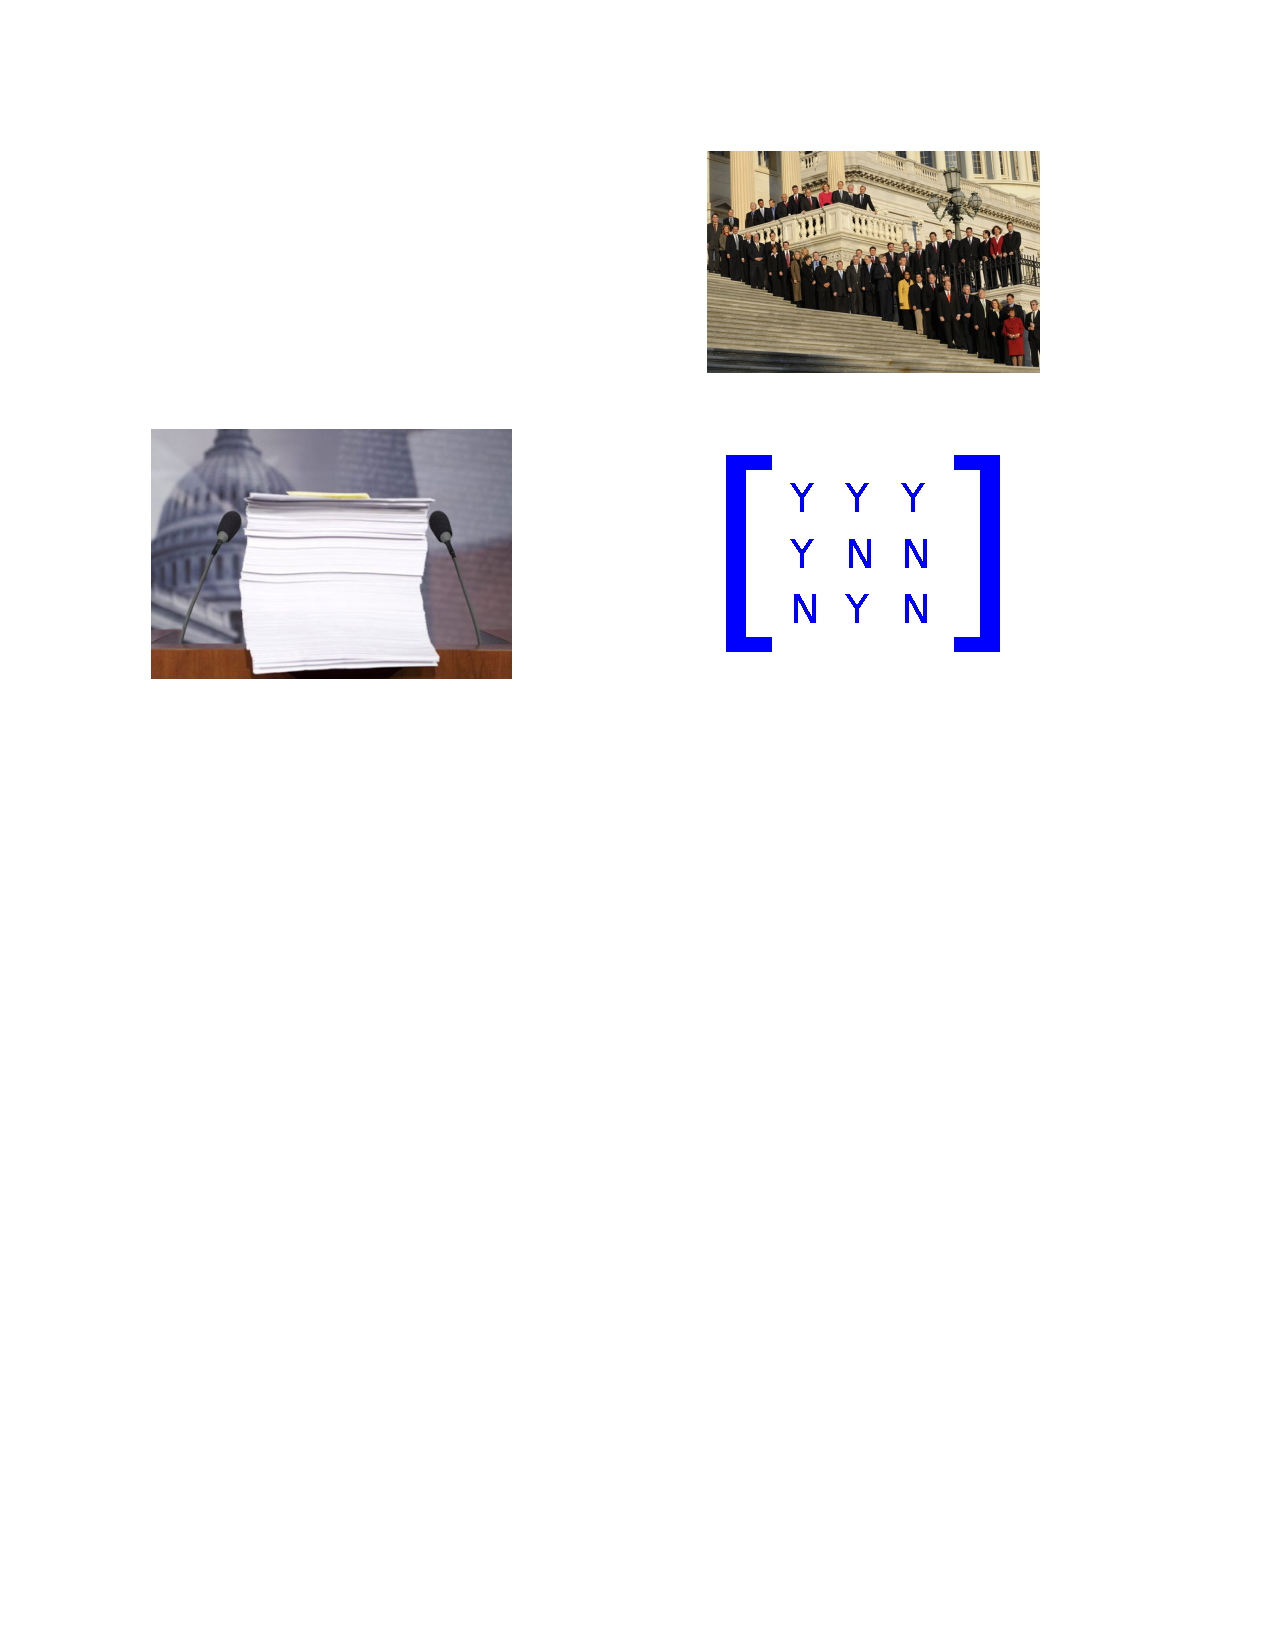
\includegraphics[width=1.0\textwidth]{figs/ideal_point_motivation_0.pdf}
% }

% \frame{
%   \frametitle{A model of voting patterns}
%   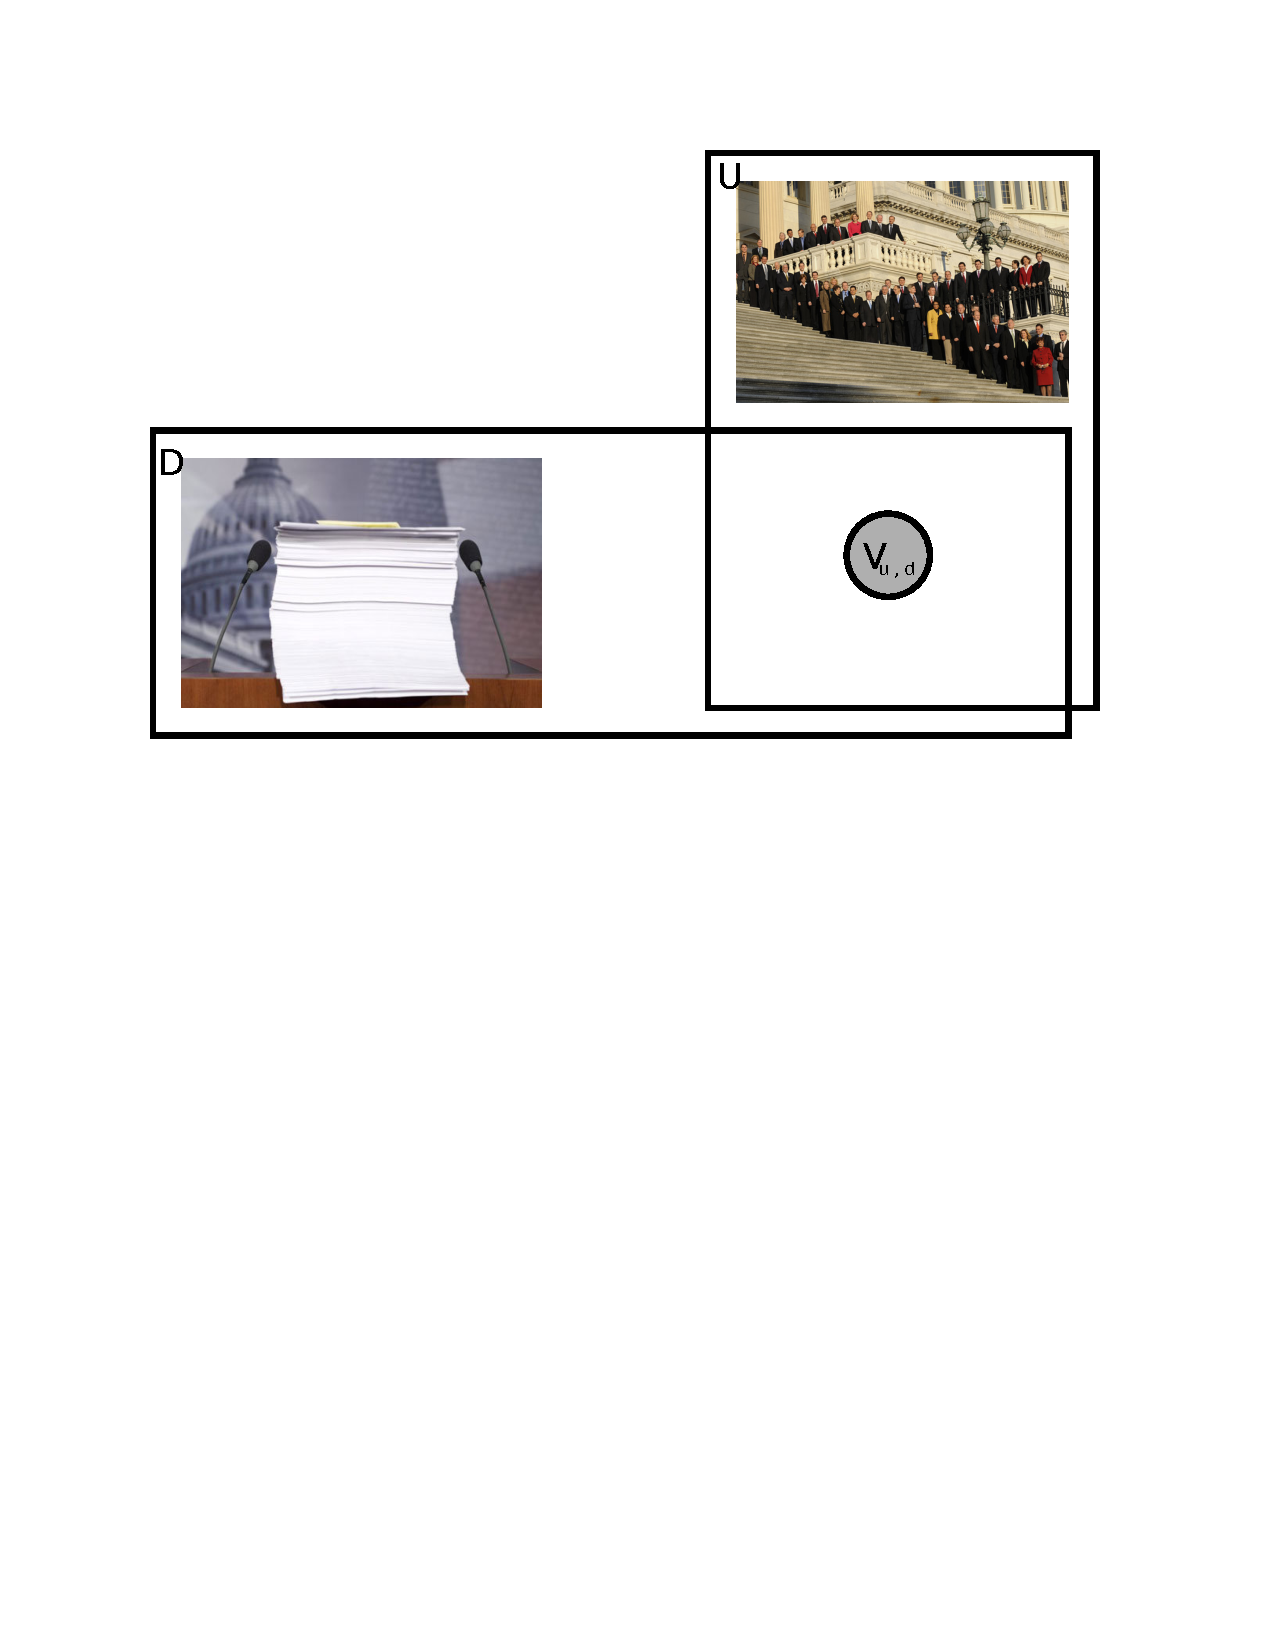
\includegraphics[width=1.0\textwidth]{figs/ideal_point_motivation_1.pdf} \\
% }

\frame{
  \frametitle{Ideal points}
  Ideal points $\textcolor{blue}{x_u}$ position lawmakers in a latent political space.
  \tiny
    \textcolor{gray}{
  \begin{tabular}{lll}
Jackman, 2001 & Poole and Rosenthal, 1985 & Martin and Quinn, 2002 \\
Jounson and Albert, 1999 & Clinton et al., 2004 & \\
  \end{tabular}
}
\normalsize
  \begin{center}
    \vspace{-120pt}
    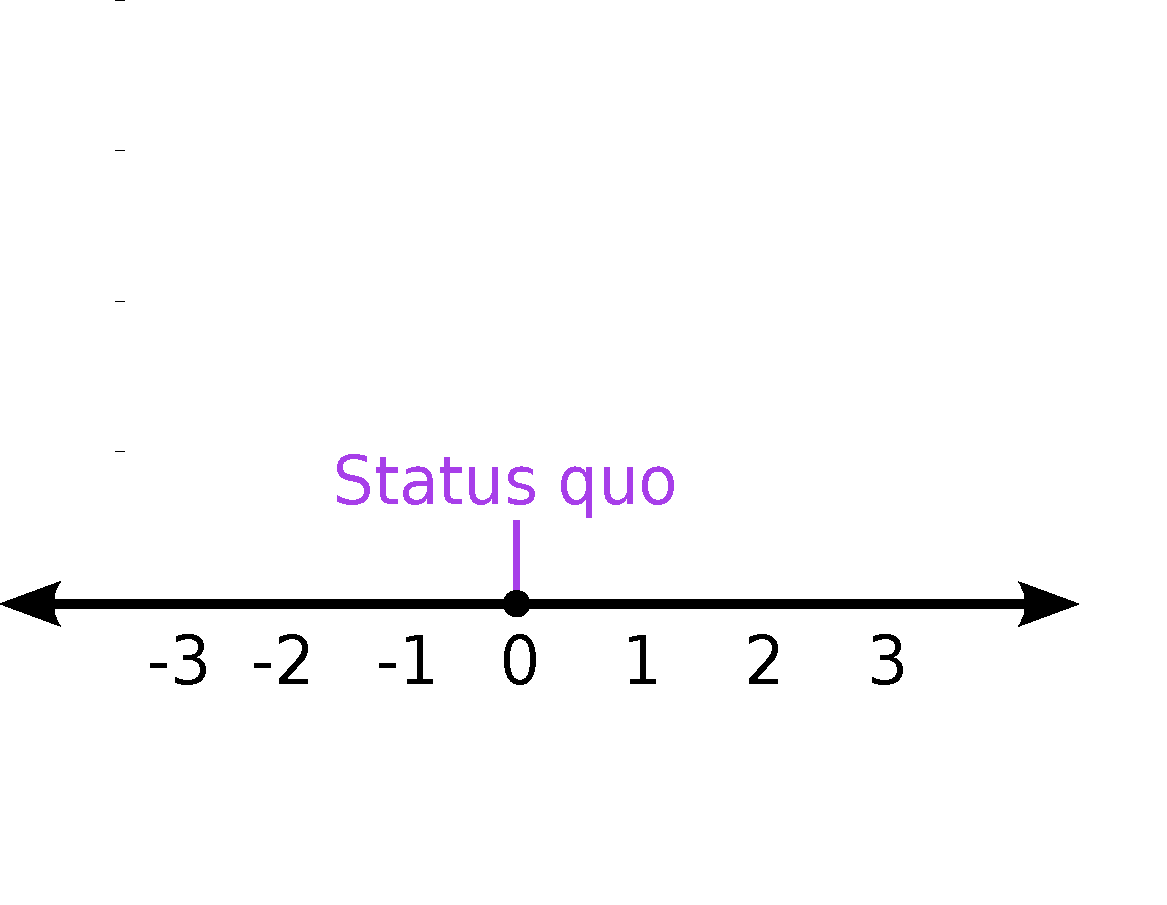
\includegraphics[scale=0.58]{figs/134_interesting_senator_name_accuracy_by_ip_sample_line.pdf}
  \end{center}
  \normalsize
}

\frame{
  \frametitle{Ideal points}
  Ideal points $\textcolor{blue}{x_u}$ position lawmakers in a latent political space.
  \tiny
    \textcolor{gray}{
  \begin{tabular}{lll}
Jackman, 2001 & Poole and Rosenthal, 1985 & Martin and Quinn, 2002 \\
Jounson and Albert, 1999 & Clinton et al., 2004 & \\
  \end{tabular}
}
\normalsize
  \begin{center}
    \vspace{-120pt}
    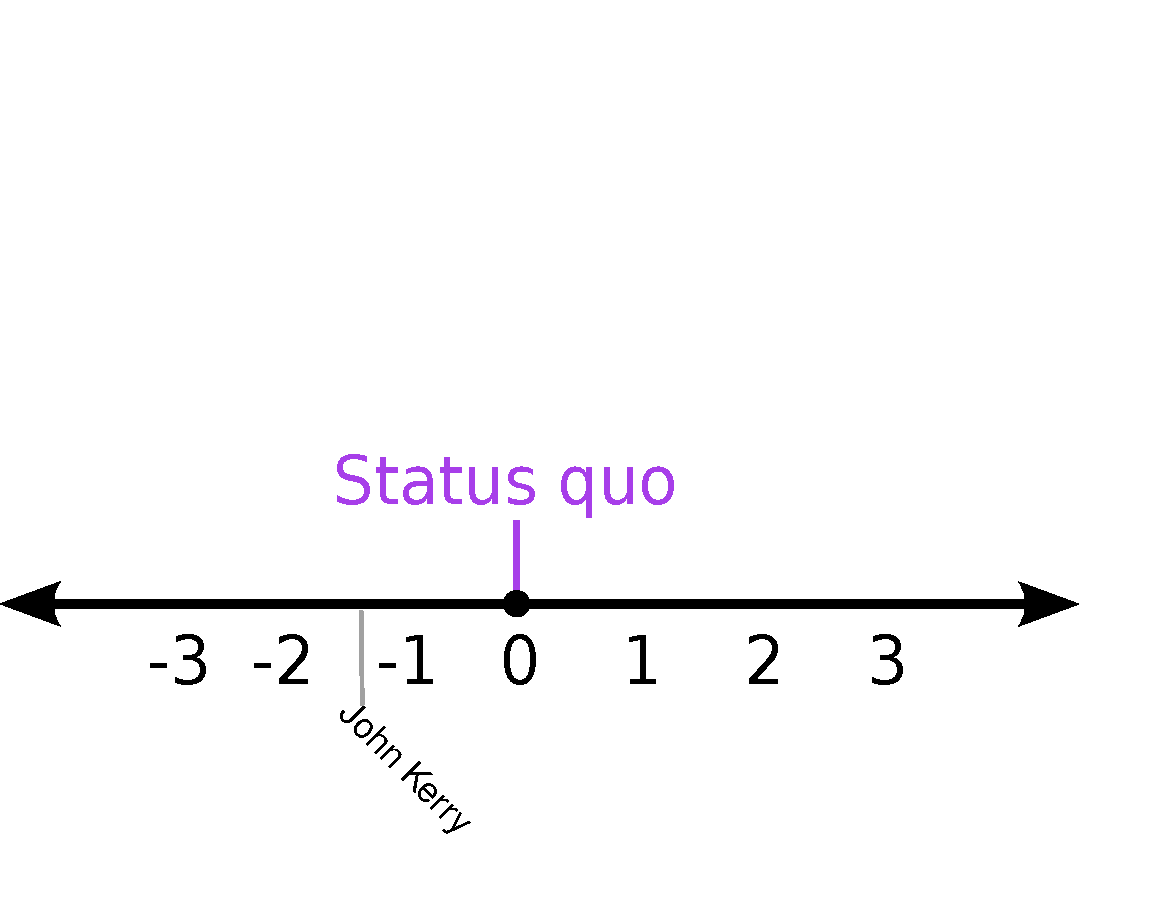
\includegraphics[scale=0.58]{figs/134_interesting_senator_name_accuracy_by_ip_sample_line_names_0.pdf}
  \end{center}
  \normalsize
}

\frame{
  \frametitle{Ideal points}
  Ideal points $\textcolor{blue}{x_u}$ position lawmakers in a latent political space.
  \tiny
    \textcolor{gray}{
  \begin{tabular}{lll}
Jackman, 2001 & Poole and Rosenthal, 1985 & Martin and Quinn, 2002 \\
Jounson and Albert, 1999 & Clinton et al., 2004 & \\
  \end{tabular}
}
\normalsize
\begin{center}
    \vspace{-120pt}
    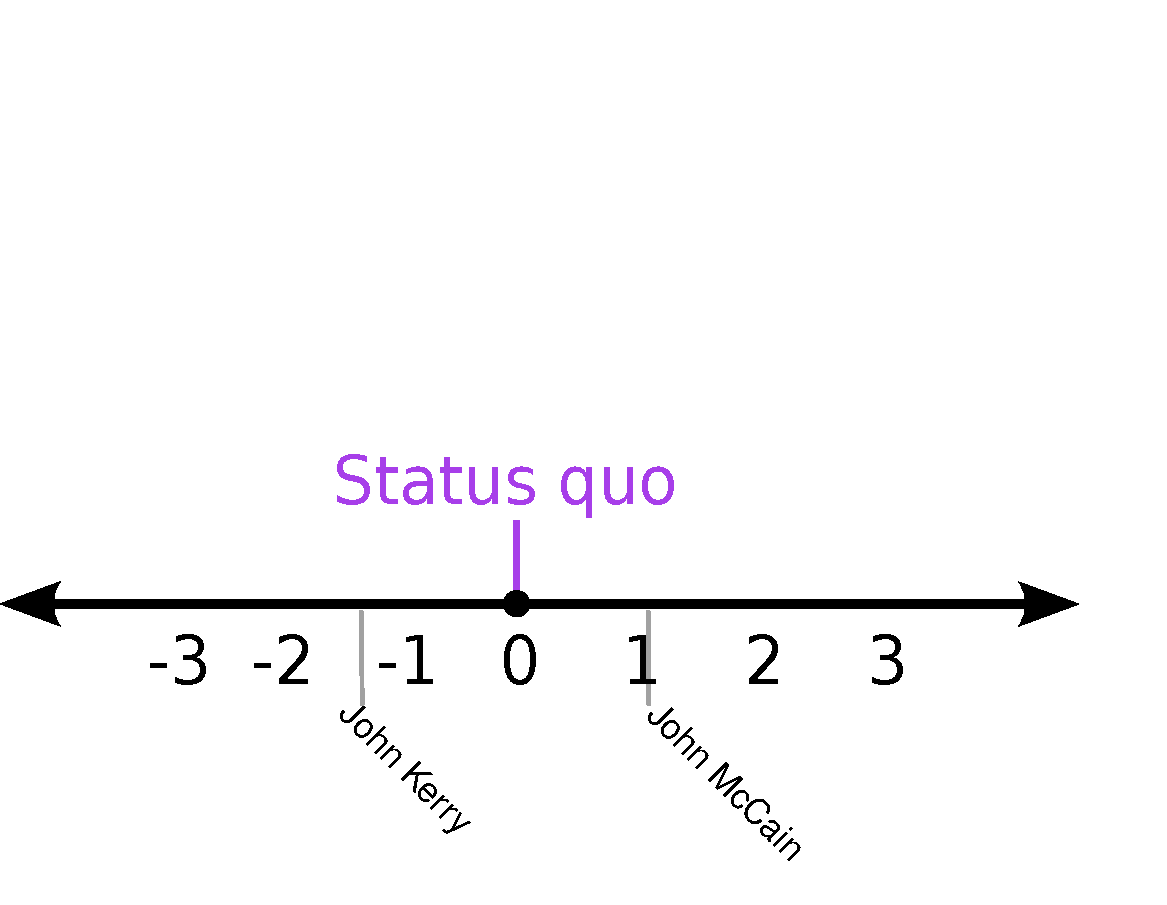
\includegraphics[scale=0.58]{figs/134_interesting_senator_name_accuracy_by_ip_sample_line_names_1.pdf}
  \end{center}
}


\frame{
  \frametitle{Ideal points}
  Ideal points $\textcolor{blue}{x_u}$ position lawmakers in a latent political space.
  \tiny
    \textcolor{gray}{
  \begin{tabular}{lll}
Jackman, 2001 & Poole and Rosenthal, 1985 & Martin and Quinn, 2002 \\
Jounson and Albert, 1999 & Clinton et al., 2004 & \\
  \end{tabular}
}
\normalsize
  \begin{center}
    \vspace{-120pt}
    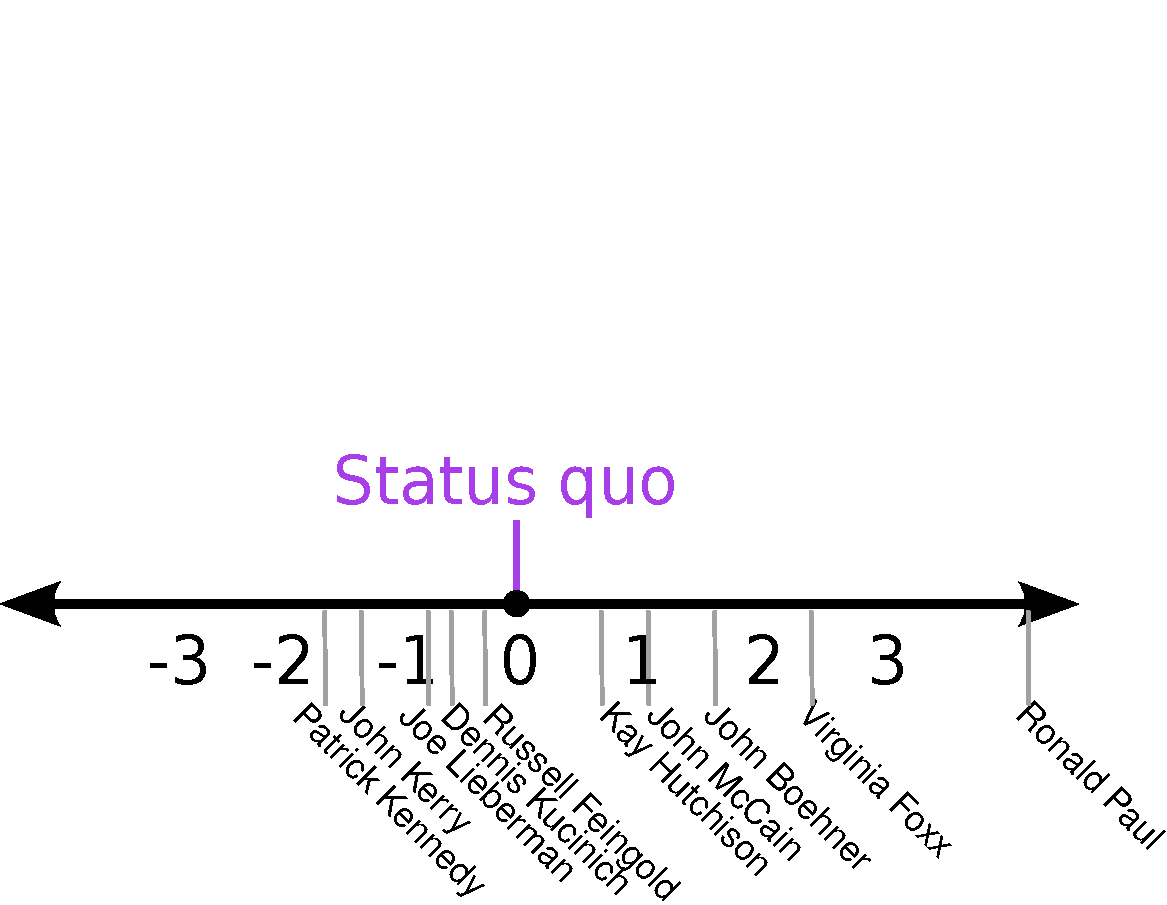
\includegraphics[scale=0.58]{figs/134_interesting_senator_name_accuracy_by_ip_sample_line_names.pdf}
  \end{center}
}


\frame{
  \frametitle{Ideal points}
  Ideal points $\textcolor{blue}{x_u}$ position lawmakers in a latent political space.
  \tiny
    \textcolor{gray}{
  \begin{tabular}{lll}
Jackman, 2001 & Poole and Rosenthal, 1985 & Martin and Quinn, 2002 \\
Jounson and Albert, 1999 & Clinton et al., 2004 & \\
  \end{tabular}
}
\normalsize
  \begin{center}
    \vspace{-120pt}  
    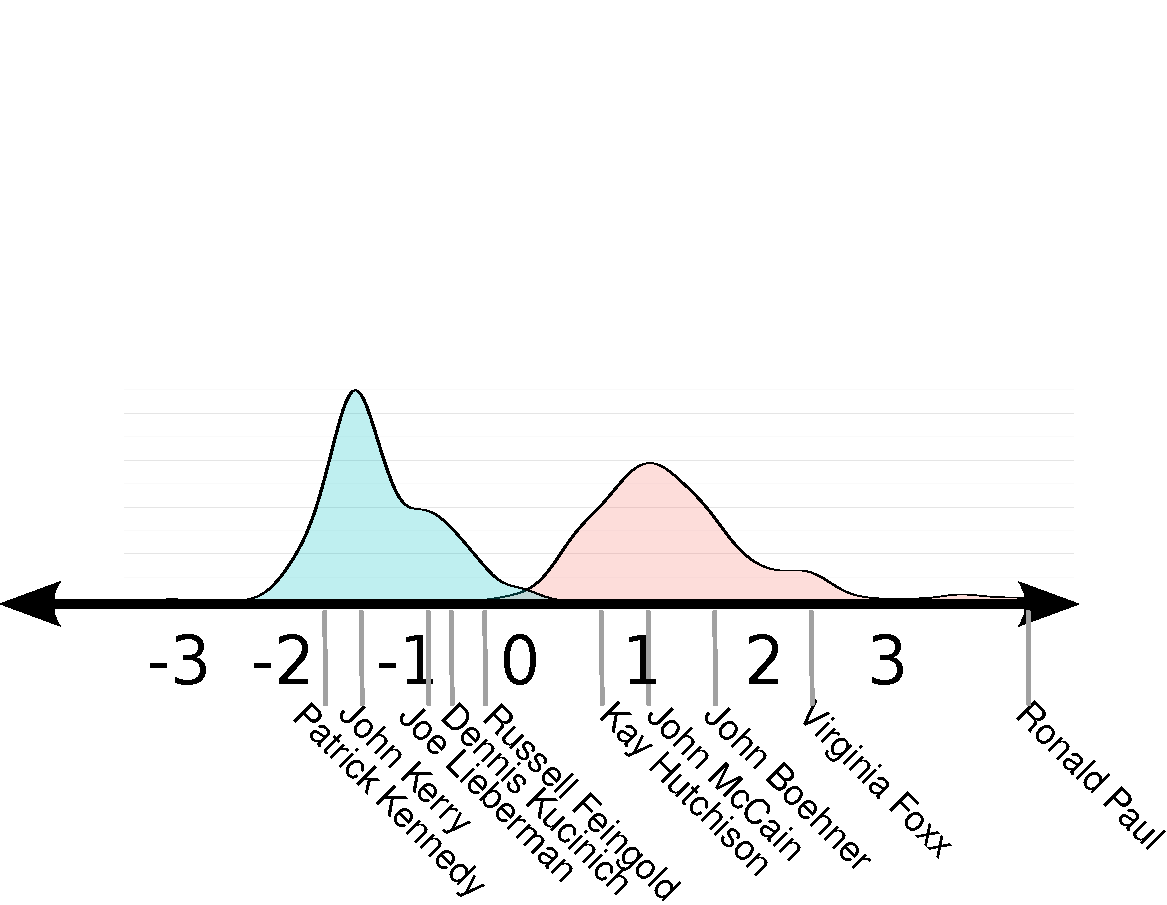
\includegraphics[scale=0.58]{figs/134_interesting_senator_name_accuracy_by_ip_sample_all.pdf}
  \end{center}
}

\frame{
  \frametitle{Documents and ideal points}
  \large
  \[ p(v_{ud} = \mbox{Yes}| x_u, \textcolor{blue}{\lambda_d}, \textcolor{blue}{\kappa_d}) = \mbox{logistic}(x_u \cdot \textcolor{blue}{\lambda_d} + \textcolor{blue}{\kappa_d}) \]
  \normalsize
%  \begin{itemize}
%    \item Discrimination $\textcolor{blue}{\lambda_d}$ describes a bill's polarity
%    \item Difficulty $\textcolor{blue}{\kappa_d}$ describes a bill's overall popularity
%    \item $ p(v_{i, j} = \mbox{Y}| x_u, \textcolor{blue}{\lambda_d}, \textcolor{blue}{\kappa_d}) = \mbox{logistic}(x_u \cdot \textcolor{blue}{\lambda_d} + \textcolor{blue}{\kappa_d})$
%  \end{itemize}
  \hspace{-20pt}
  \vspace{-20pt}
    \begin{tabular}{rll}
  \onslide<1->{
    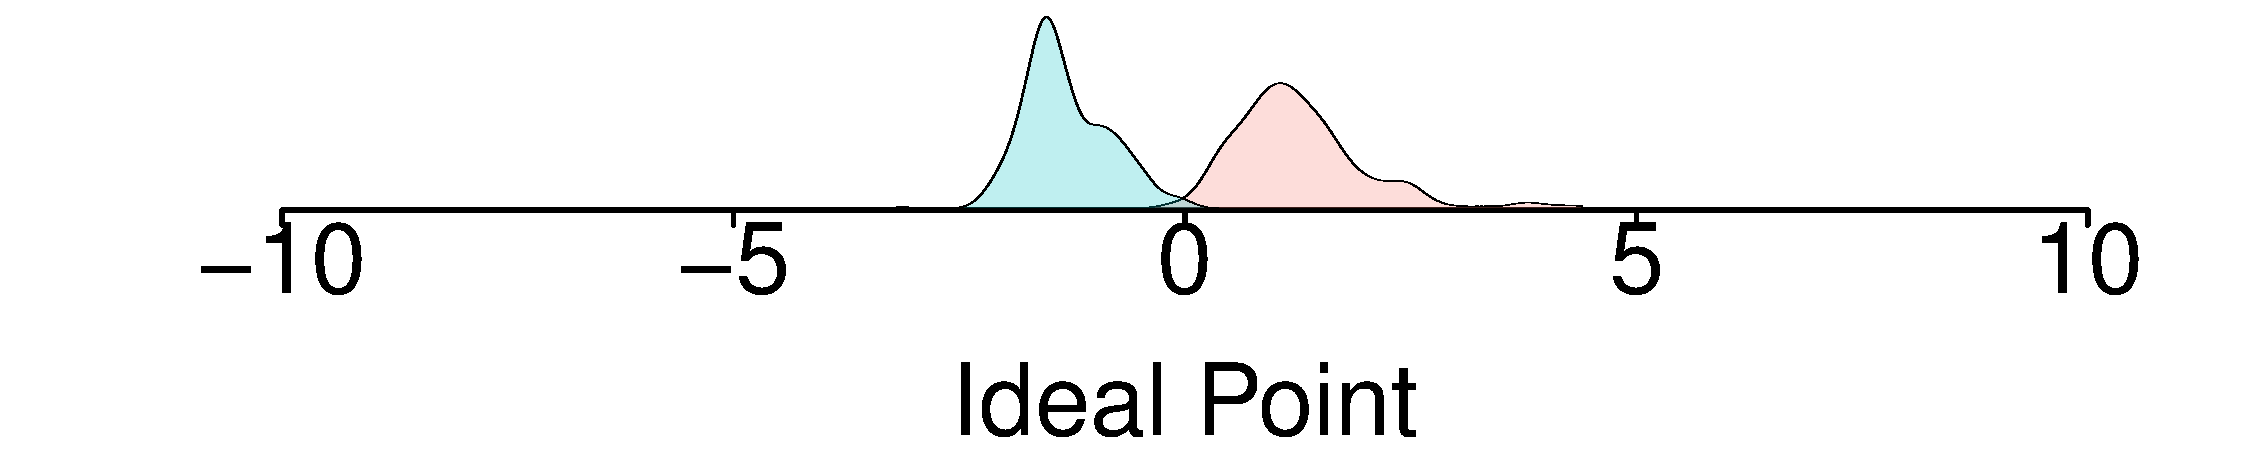
\includegraphics[width=0.7\textwidth]{figs/logistic_intro.pdf} &
    $\textcolor{white}{\lambda_d=1}$ & $\textcolor{white}{\kappa_d=0}$ \\
  }\newline
  \vspace{5pt}
  \onslide<1->{
    
\includegraphics[width=0.7\textwidth]{figs/logistic_blank.pdf} &
    $\textcolor{white}{\lambda_d=20}$ & $\textcolor{white}{\kappa_d=0}$ \\
  }
  \vspace{5pt}
  \onslide<1->{
    
\includegraphics[width=0.7\textwidth]{figs/logistic_blank.pdf} &
    $\textcolor{white}{\lambda_d=-0.4}$ & $\textcolor{white}{\kappa_d=2}$ \\
  }
  \vspace{5pt}
  \onslide<1->{
    
\includegraphics[width=0.7\textwidth]{figs/logistic_blank.pdf} &
    $\textcolor{white}{\lambda_d=1}$ & $\textcolor{white}{\kappa_d=-5}$ \\
  }
  \end{tabular}

}

\frame{
  \frametitle{Documents and ideal points}
%  \begin{itemize}
%    \item Discrimination $\textcolor{blue}{\lambda_d}$ describes a bill's polarity
%    \item Difficulty $\textcolor{blue}{\kappa_d}$ describes a bill's overall popularity
%    \item
  \large
  \[ p(v_{ud} = \mbox{Yes}| x_u, \textcolor{blue}{\lambda_d}, \textcolor{blue}{\kappa_d}) = \mbox{logistic}(x_u \cdot \textcolor{blue}{\lambda_d} + \textcolor{blue}{\kappa_d}) \]
  \normalsize
%  \end{itemize}
  \hspace{-20pt}
  \vspace{-20pt}
    \begin{tabular}{rll}
  \onslide<1->{
    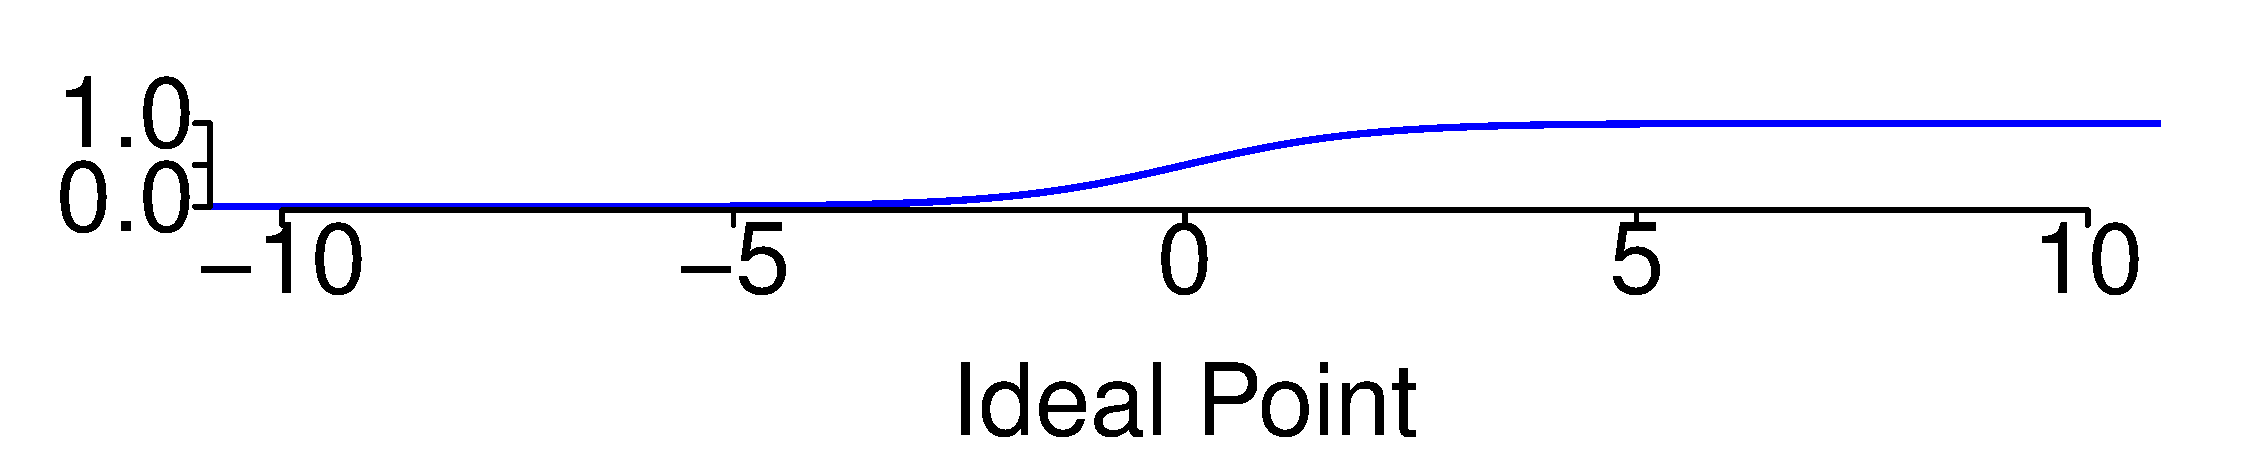
\includegraphics[width=0.7\textwidth]{figs/logistic_1_0.pdf} &
    $\lambda_d=1$ & $\kappa_d=0$ \\
  }\newline
  \vspace{5pt}
  \onslide<2->{
    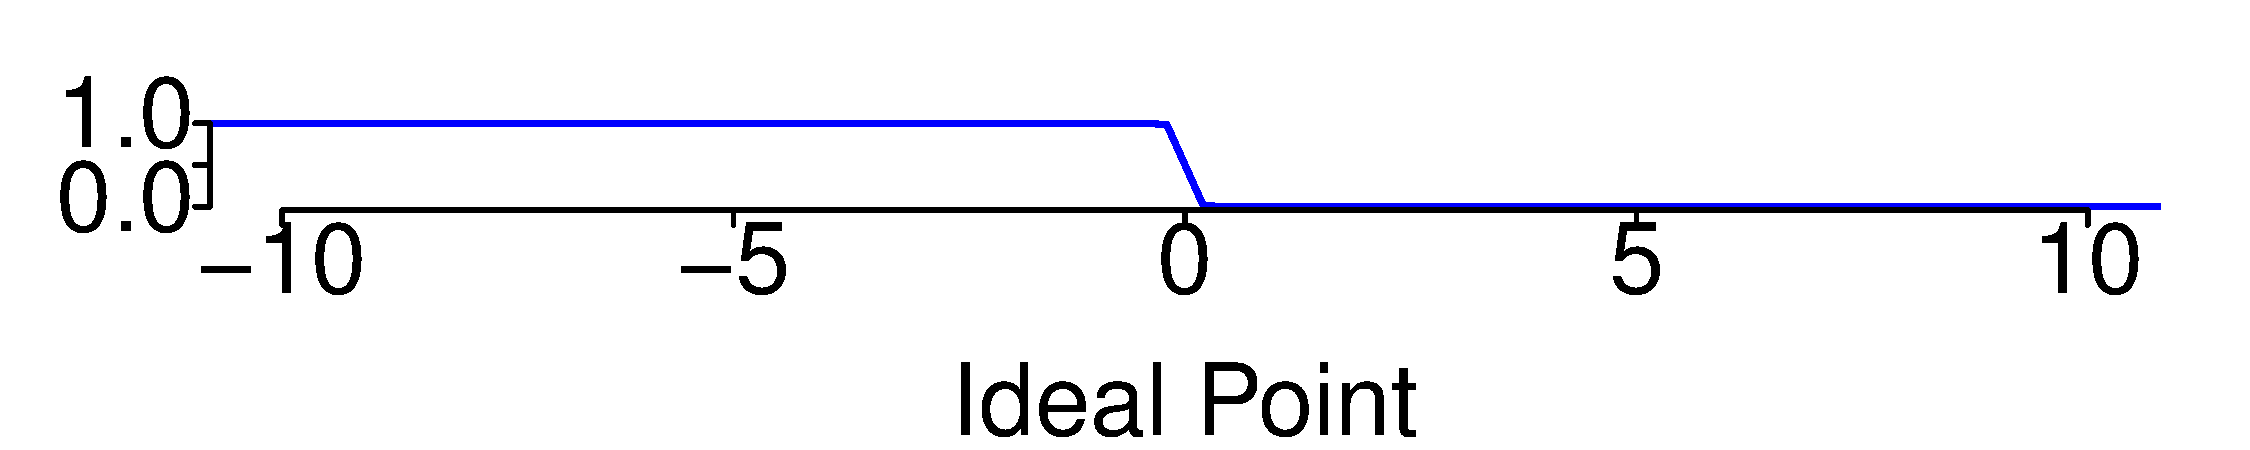
\includegraphics[width=0.7\textwidth]{figs/logistic_n20_0.pdf} &
    $\lambda_d=-20$ & $\kappa_d=0$ \\
  }
  \vspace{5pt}
  \onslide<3->{
    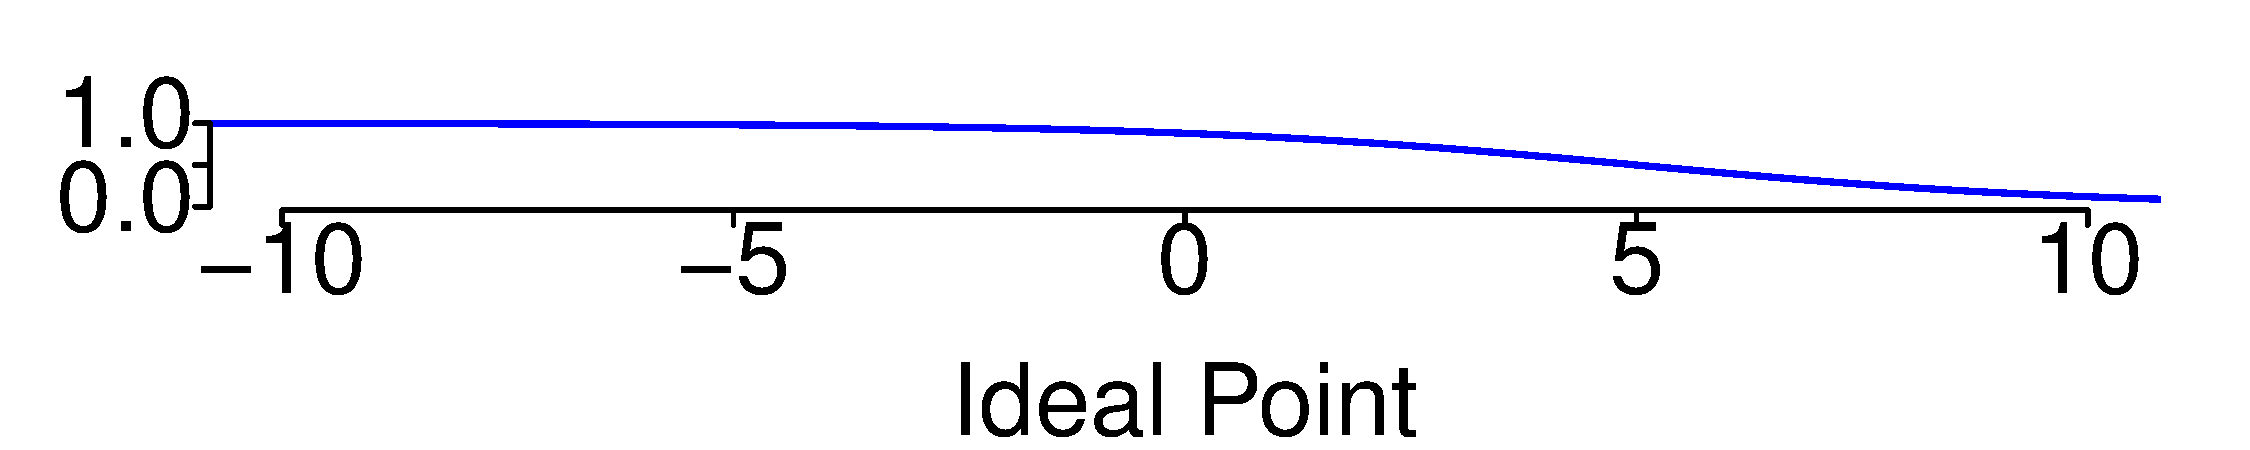
\includegraphics[width=0.7\textwidth]{figs/logistic_np4_2.pdf} &
    $\lambda_d=-0.4$ & $\kappa_d=2$ \\
  }
  \vspace{5pt}
  \onslide<4->{
    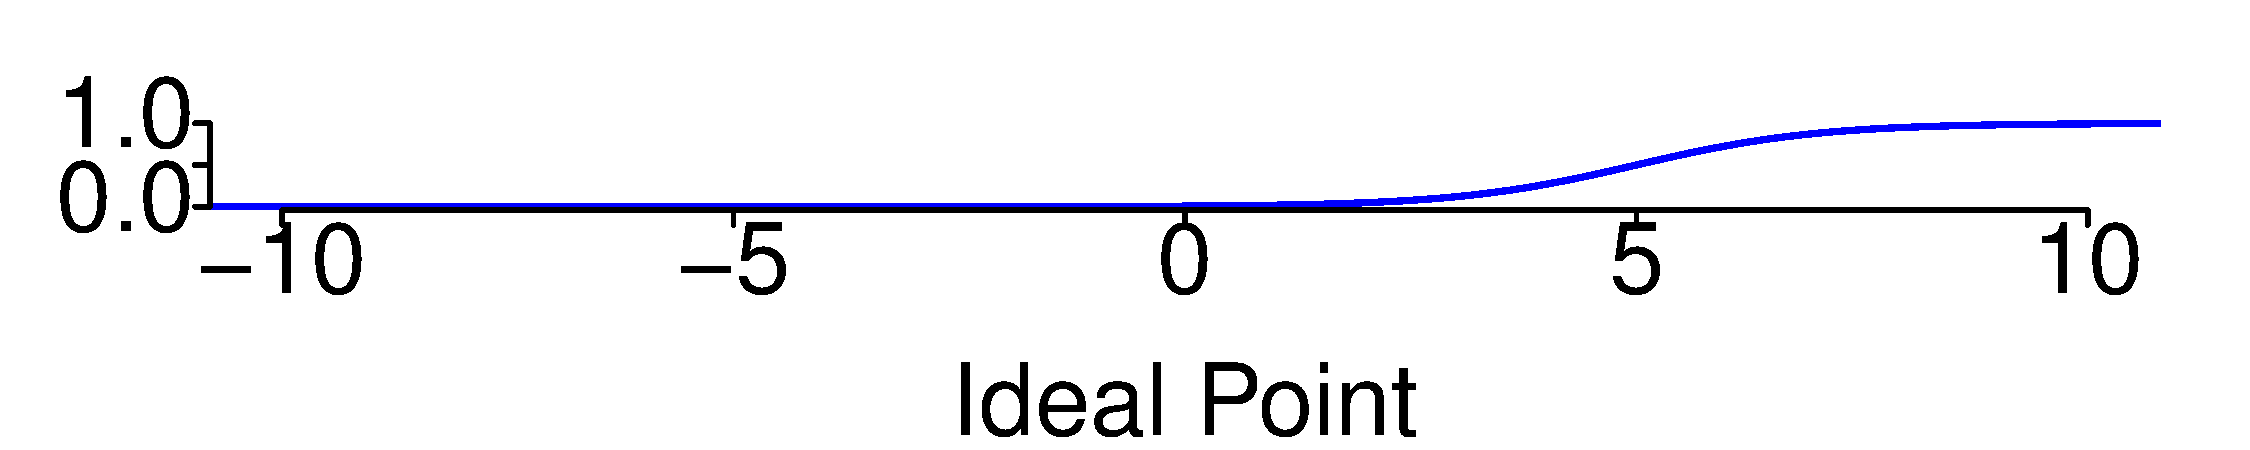
\includegraphics[width=0.7\textwidth]{figs/logistic_1_n5.pdf} &
    $\lambda_d=1$ & $\kappa_d=-5$ \\
  }
  \end{tabular}
}

\frame{
  \frametitle{The Ideal Point Model}
  \tiny
    \textcolor{gray}{
  \begin{tabular}{lll}
Jackman, 2001 & Poole and Rosenthal, 1985 & Martin and Quinn, 2002 \\
Jounson and Albert, 1999 & Clinton et al., 2004 & \\
  \end{tabular}
}
  \large
  \begin{align*}
  \hspace{-40pt}
    p(v_{ud} = \mbox{Yes}| x_u, \lambda_d, \kappa_d) = \mbox{logistic}(x_u \cdot \lambda_d + \kappa_d) \\
  \end{align*}
  \normalsize
  \vspace{-50pt}
  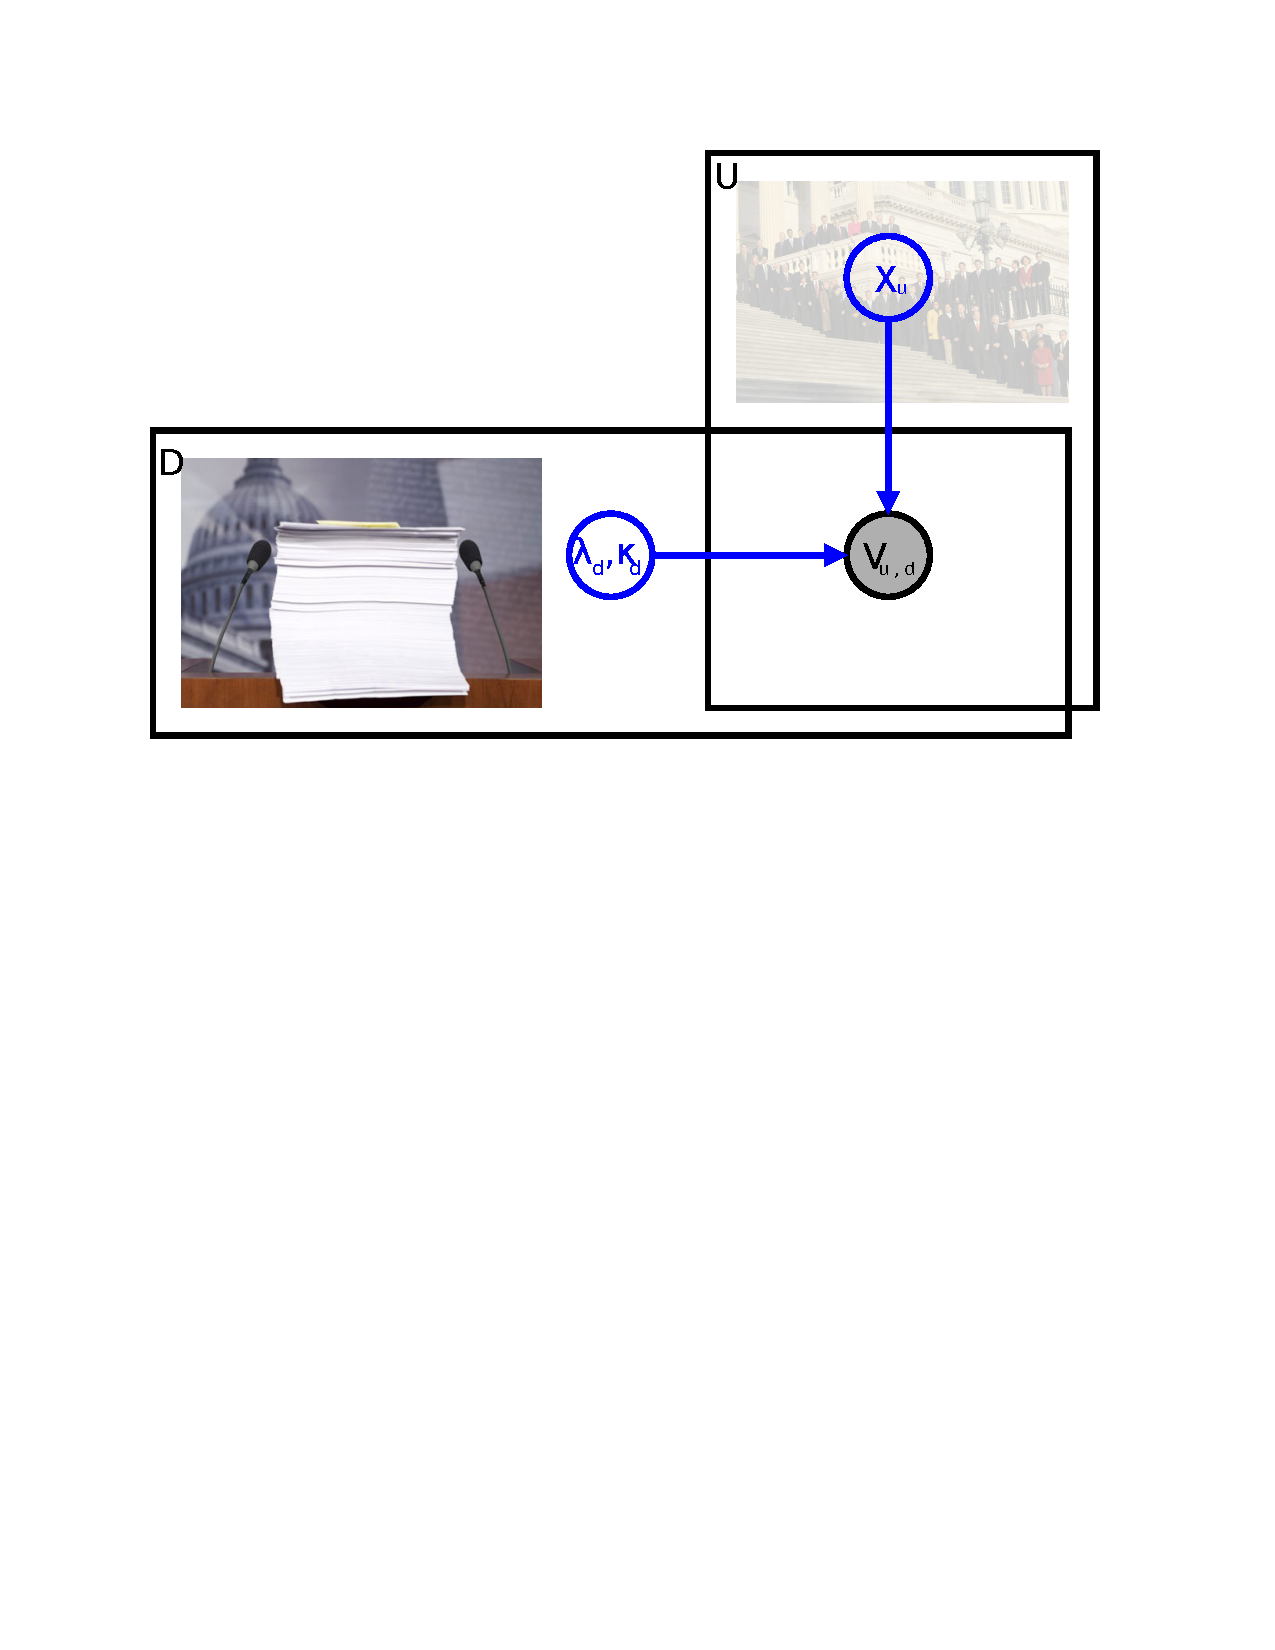
\includegraphics[width=1\textwidth]{figs/ideal_point_motivation_2.pdf} \\
}

\frame{
  \frametitle{Adding text to the ideal point model}
  \normalsize
  We can use the text of legislation to infer bills' positions.
  \large
  \begin{eqnarray*}
    \textcolor{white}{\lambda_d \sim \mathcal{N}(\bm \eta_{\lambda}^T \bm w_d, \sigma^2)} \\
    \textcolor{white}{\kappa_d \sim \mathcal{N}(\bm \eta_{\kappa}^T \bm w_d, \sigma^2)} \\
  \end{eqnarray*}
  \normalsize
  \vspace{-60pt}
  \center
  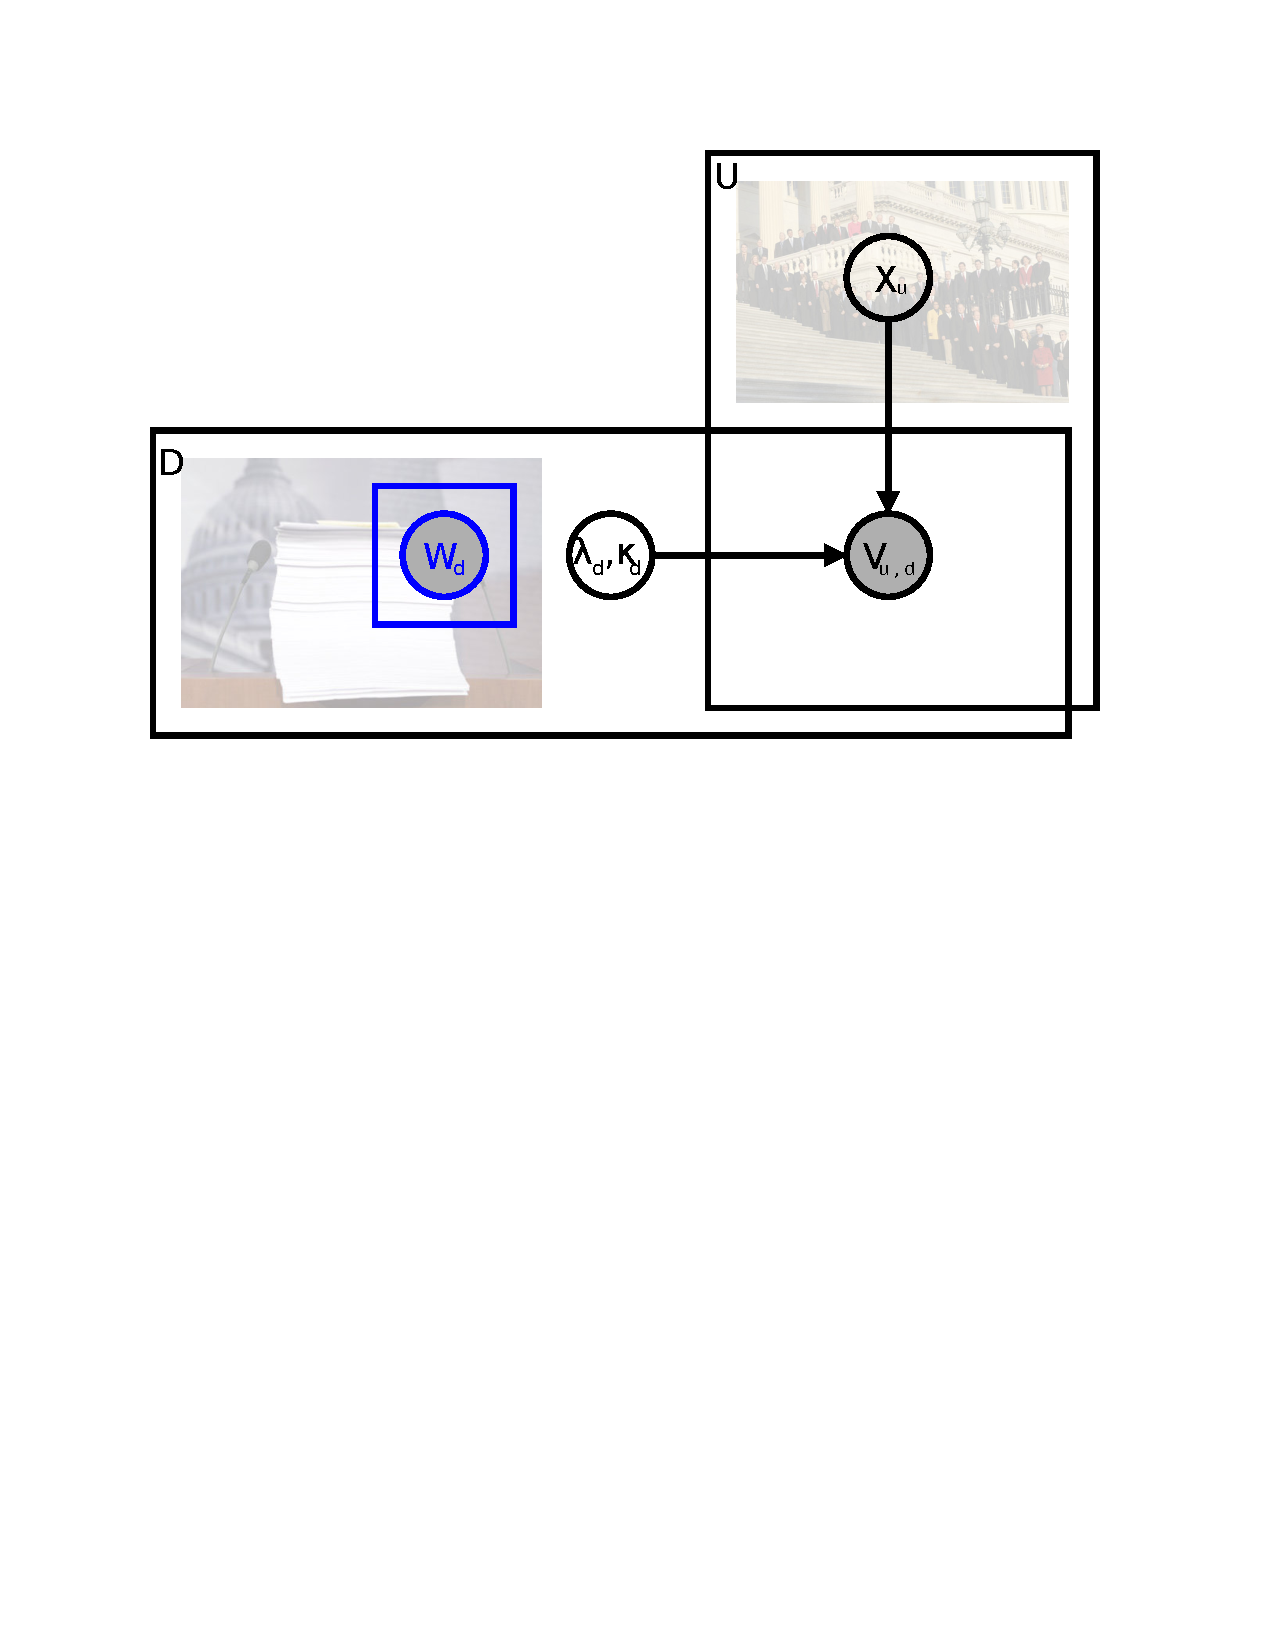
\includegraphics[width=1\textwidth]{figs/ideal_point_motivation_3.pdf}
  \vspace{-20pt} \textcolor{white}{We regularize ${\bm \eta}$ using both ridge and lasso penalties.}
}

\frame{
  \frametitle{Ideal Point Text Regression}
  Regress document parameters on word counts:
  \large
  \begin{eqnarray*}
    \lambda_d \sim \mathcal{N}(\bm \eta_{\lambda}^T \bm w_d, \sigma^2) \\
    \kappa_d \sim \mathcal{N}(\bm \eta_{\kappa}^T \bm w_d, \sigma^2) \\
  \end{eqnarray*}
  \normalsize
  \vspace{-60pt} 
  \center
  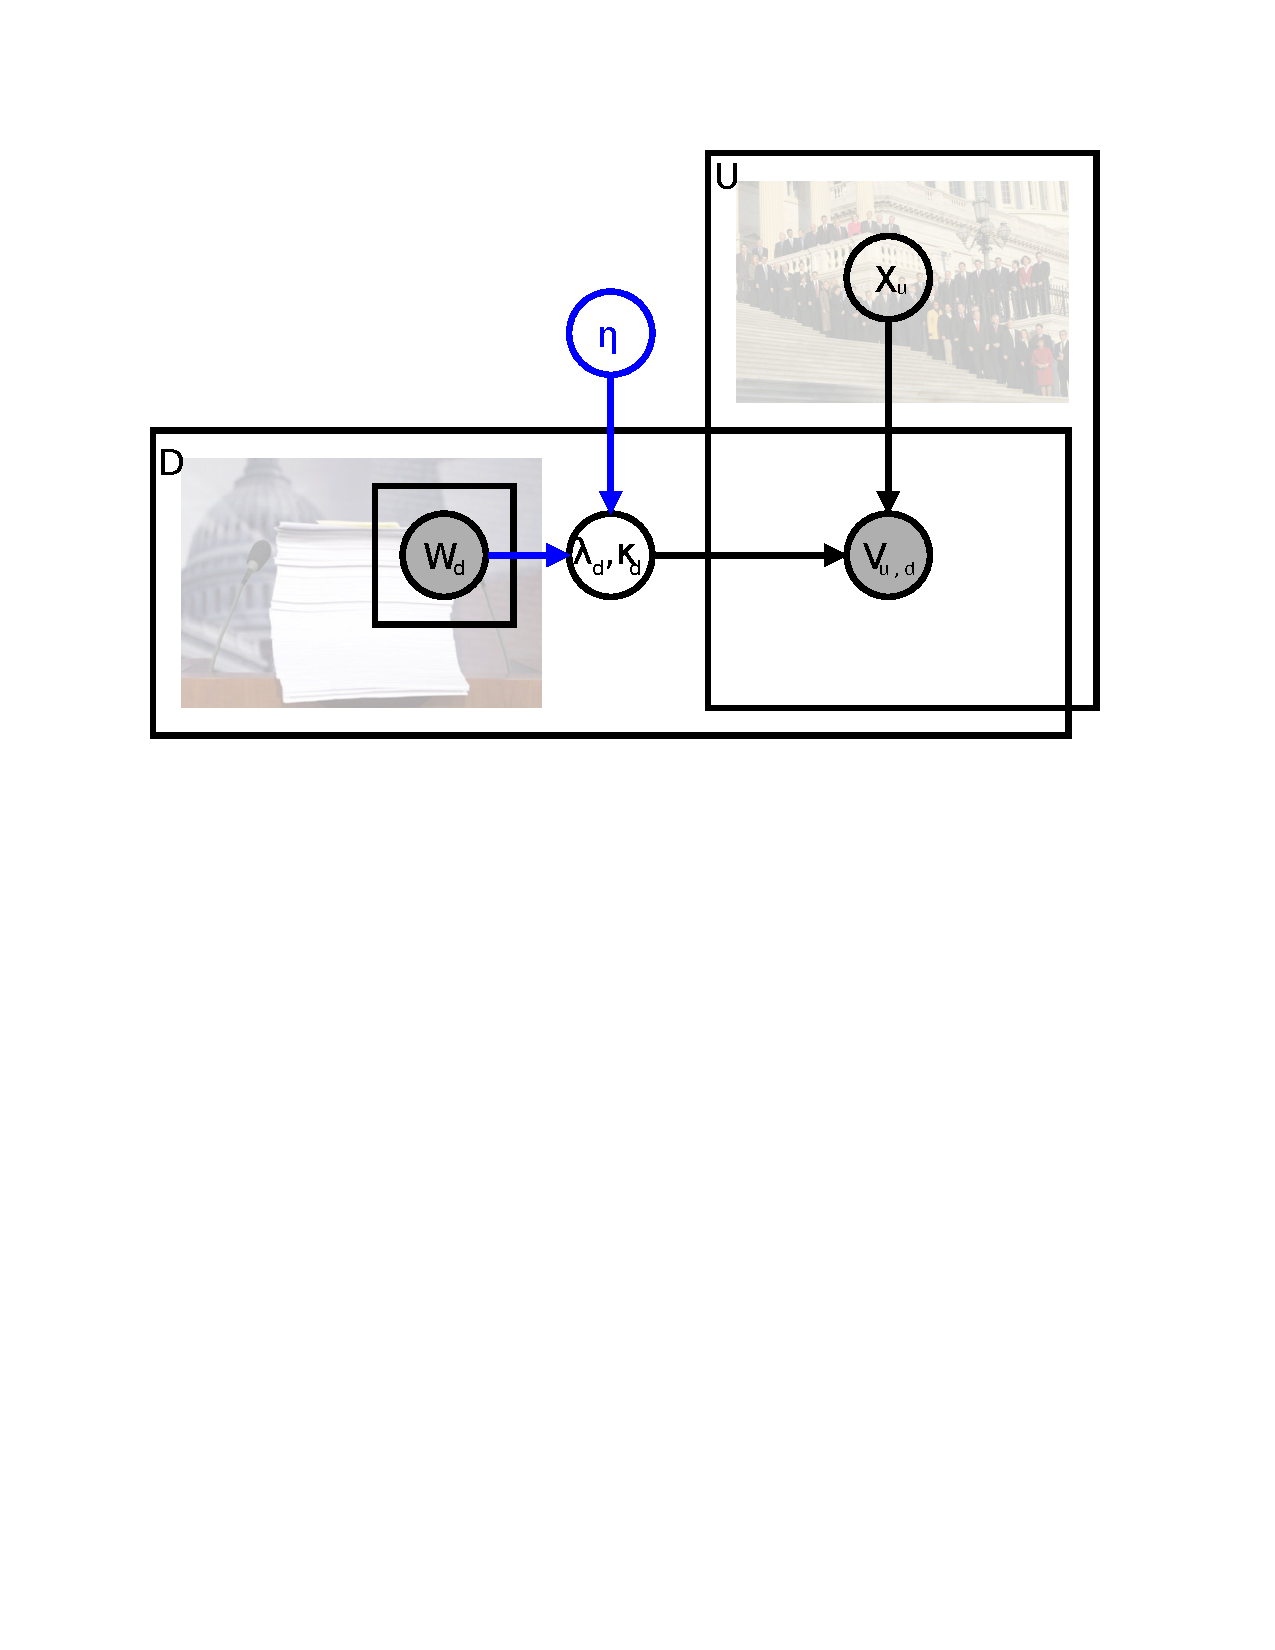
\includegraphics[width=1.0\textwidth]{figs/ideal_point_text_regression.pdf} \\
  \vspace{-20pt} We regularize ${\bm \eta}$ using both ridge and lasso penalties.
}

\frame{
  \frametitle{Ideal Point Topic modeling}
  Use supervised topics to infer document parameters. \small \textcolor{gray}{Blei et al. 2008} \\
  \large
  \vspace{30pt}
  \center
  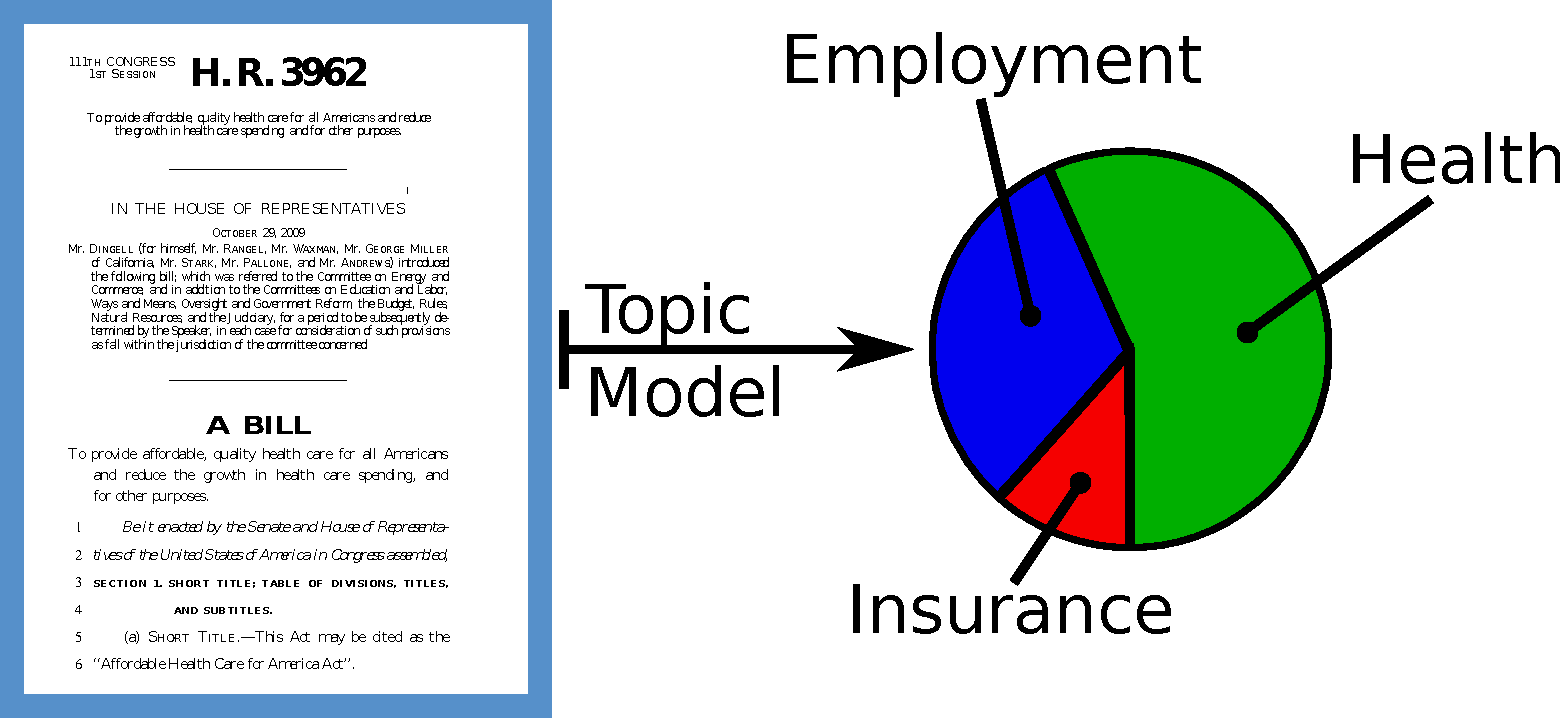
\includegraphics[width=0.90\textwidth]{figs/topics.pdf}

}

\frame{
  \frametitle{Ideal Point Topic modeling}
  Use supervised topics to infer document parameters. \small \textcolor{gray}{Blei et al. 2008}
  \large
  \begin{eqnarray*}
  \lambda_d \sim \mathcal{N}({\bm \eta_{\lambda}^T} \bar {\bm z_d}, \sigma^2) \\
  \kappa_d \sim \mathcal{N}({\bm \eta_{\kappa}^T} \bar {\bm z_d}, \sigma^2) \\
  \end{eqnarray*}
  \normalsize
  \vspace{-60pt}
  \center
  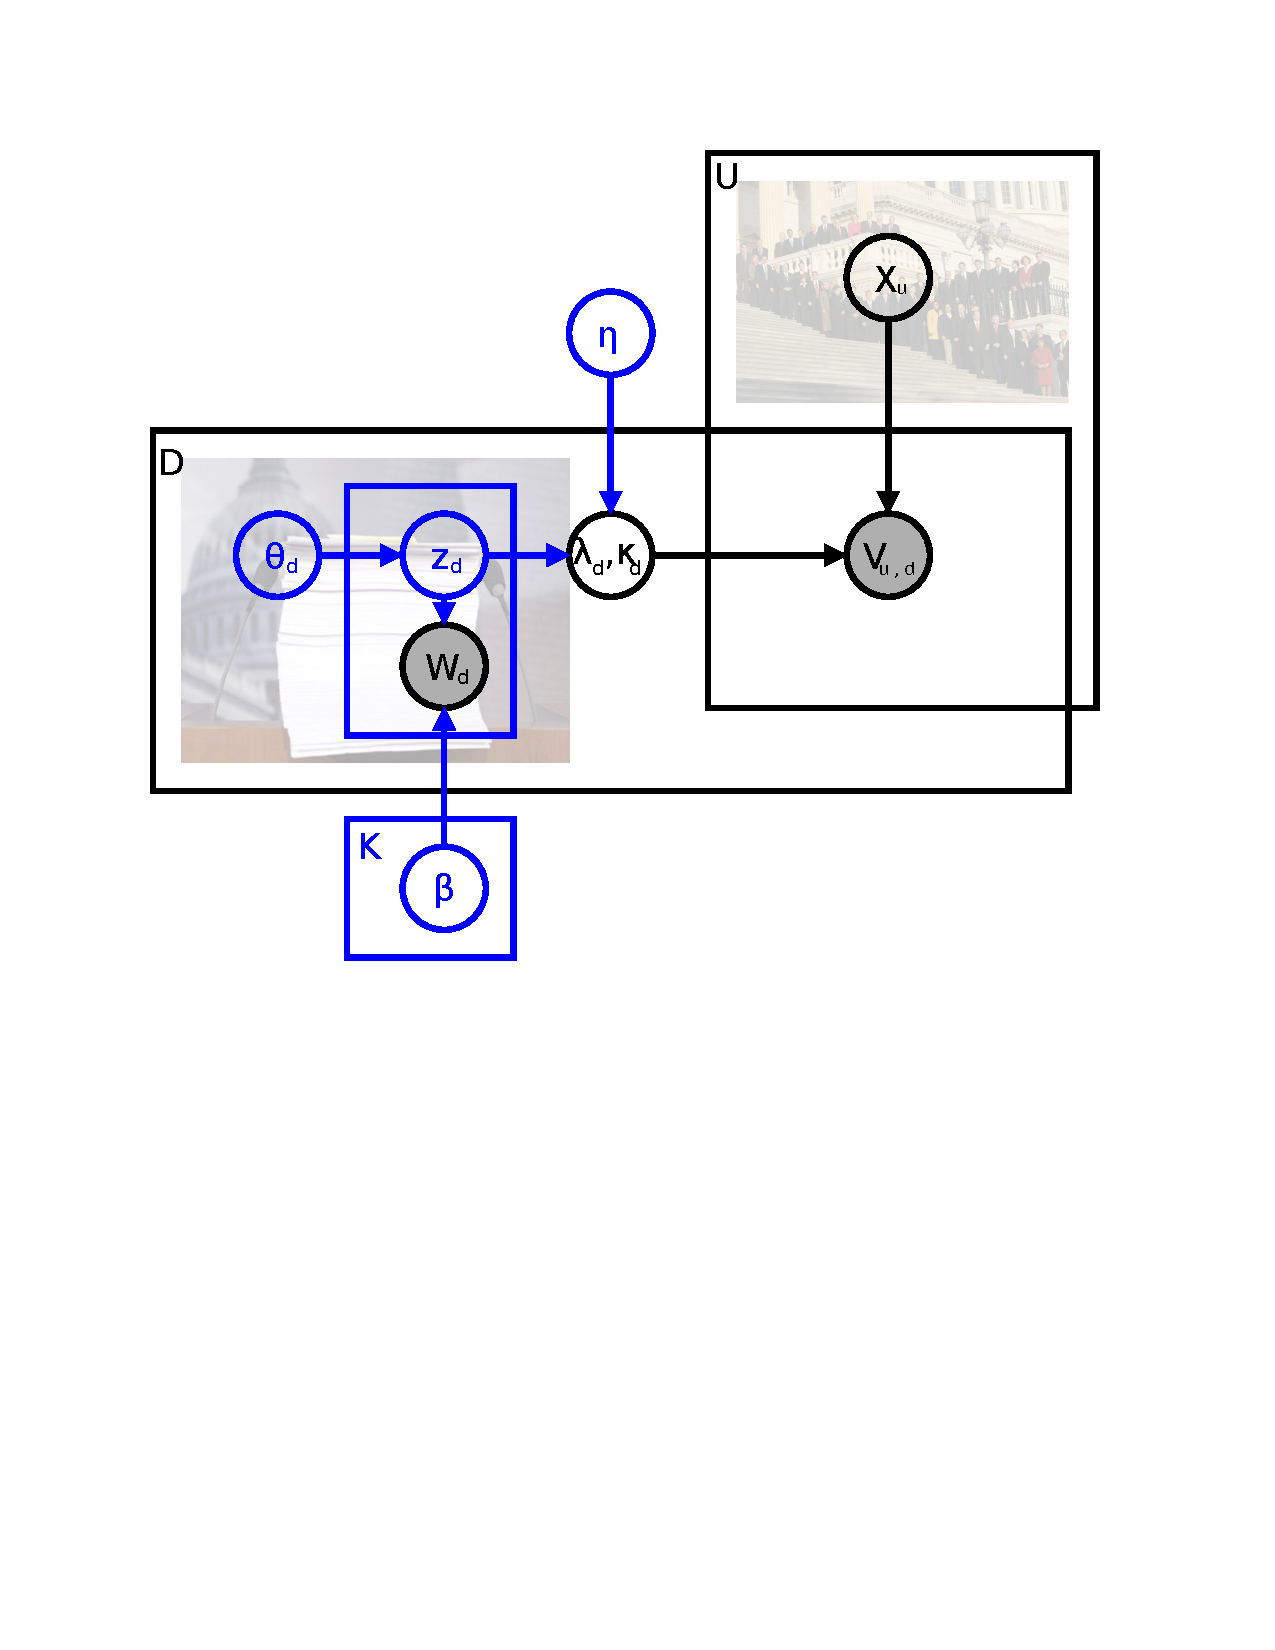
\includegraphics[width=0.74\textwidth]{figs/ideal_point_topic_model.pdf}
  \vspace{-20pt} Topics adjust as regression parameters $\bm \eta$ are fit
}


\frame{
  \frametitle{Posterior Inference}
  Recall that we only observe words $\bm W$ and votes $V$. \\
  We are interested in the posterior
  \begin{eqnarray*}
    p(\lambda_d, \kappa_d, x_u, \bm \eta | V, \bm W)
  \end{eqnarray*}
  We derived a mean-field variational inference algorithm.
  \begin{itemize}
    \item This involves positing a family of fully factorized posterior distributions and finding the distribution from this family which is ``closest'' in K-L divergence to the true posterior.
    \item The resulting ideal points are correlated at over 0.98
      with MCMC ideal points (the standard in this field).
    \item Variational methods like this are amenable to inference in large-scale datasets. \small \textcolor{gray}{Hoffman et al. 2010} \normalsize
  \end{itemize}
%  \begin{center}
%  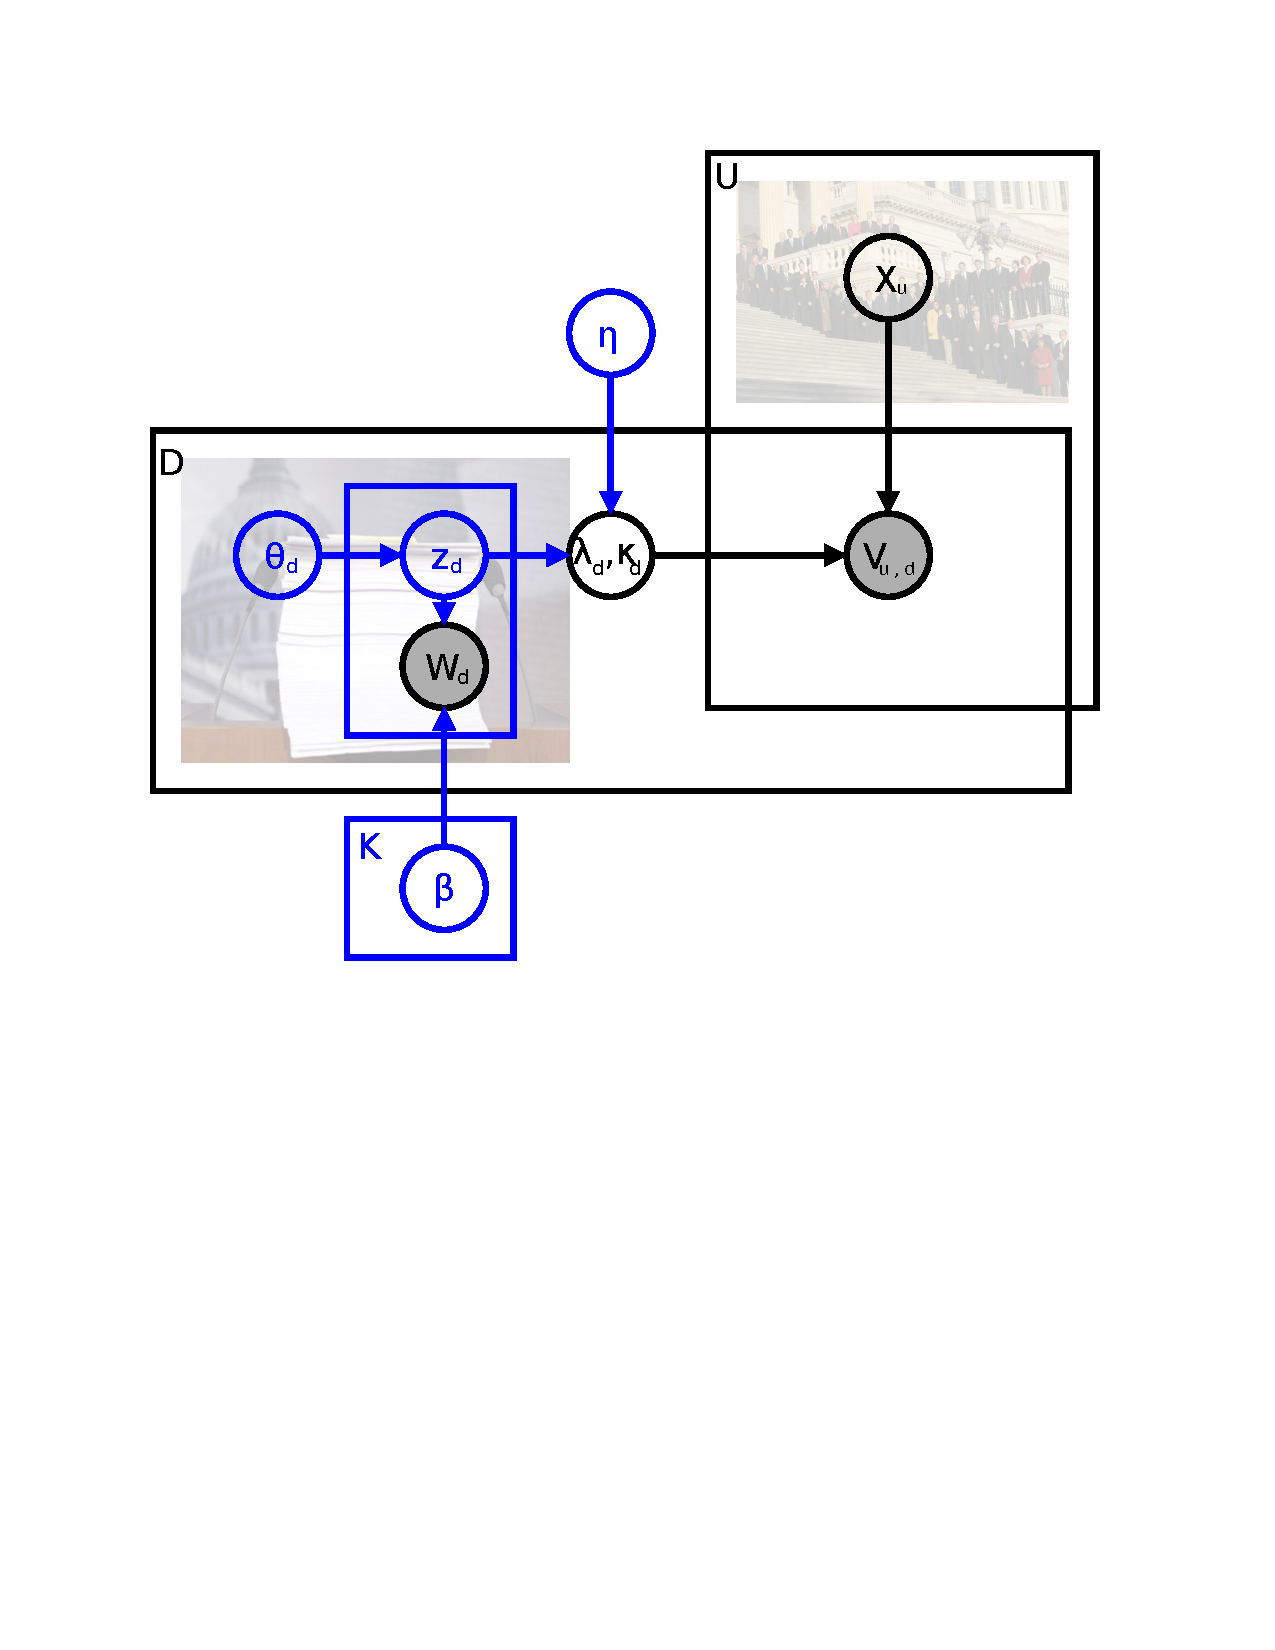
\includegraphics[width=0.5\textwidth]{figs/ideal_point_topic_model.pdf} \\
%  \end{center}

}

\frame{
  \frametitle{Derivation and implementation of variational inference}
  Finding the variational posterior involves optimizing a lower bound on the model evidence $p(V, \bm W)$. \\
  \vspace{6pt}
  This objective is optimized via gradient ascent, and we can use a few tricks to find the objective and converge better, e.g.: \\
  \begin{itemize}
    \item Use a second-order delta approximation for the bound \small \textcolor{gray}{Bickel et al. 2007} \normalsize
    \item Update subsets of lawmakers and legislation in a round-robin fashion to avoid cycles
    \end{itemize}
}

\frame{
  \frametitle{Experiments}
  \begin{itemize}
    \item We fit this model to each congressional session
      (2-year period) from to Jan 1997 to Jan 2011. \\
      \vspace{6pt}
    \item Data is from Govtrack.us \\
      \vspace{6pt}
    \item There were: \\
      \vspace{6pt}
      \begin{itemize}
      \item 4,447 bills \\
      \vspace{6pt}
      \item 1,269 lawmakers \\
      \vspace{6pt}
      \item 1,837,033 yea/nay roll-call votes \\
    \end{itemize}  
  \end{itemize}
}

\frame{
  \begin{tabular}{c}
    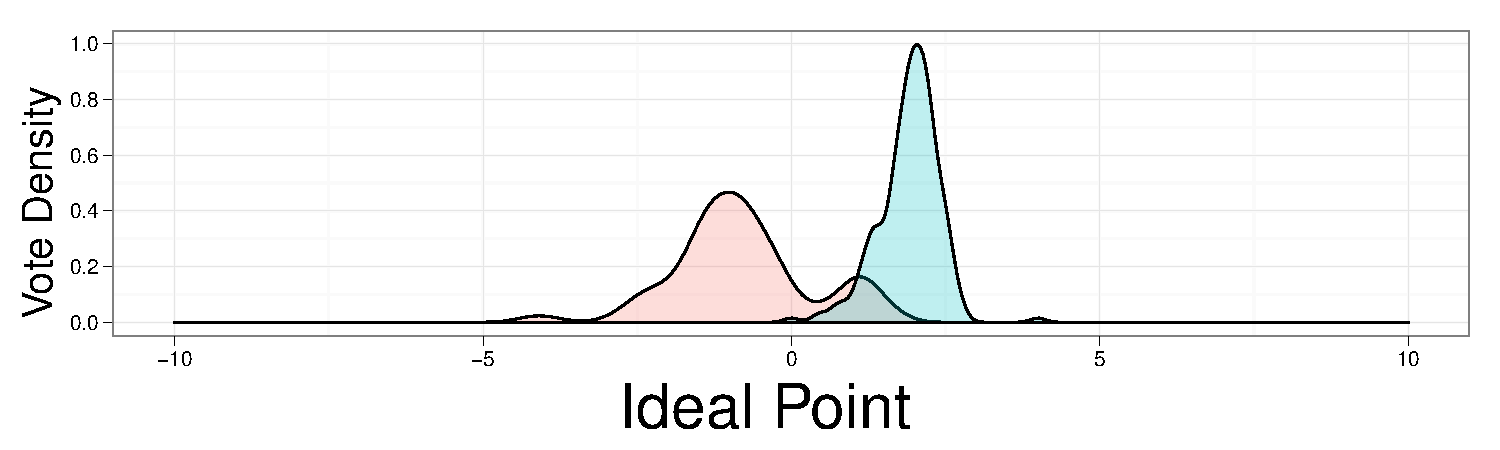
\includegraphics[width=0.8\textwidth]{figs/health_care_ideal_point.pdf}
  \end{tabular}
  \begin{columns}
    \begin{column}{0.3\textwidth}
%      \setlength\fboxsep{4pt}
%      \setlength\fboxrule{0.5pt}
%    \fbox{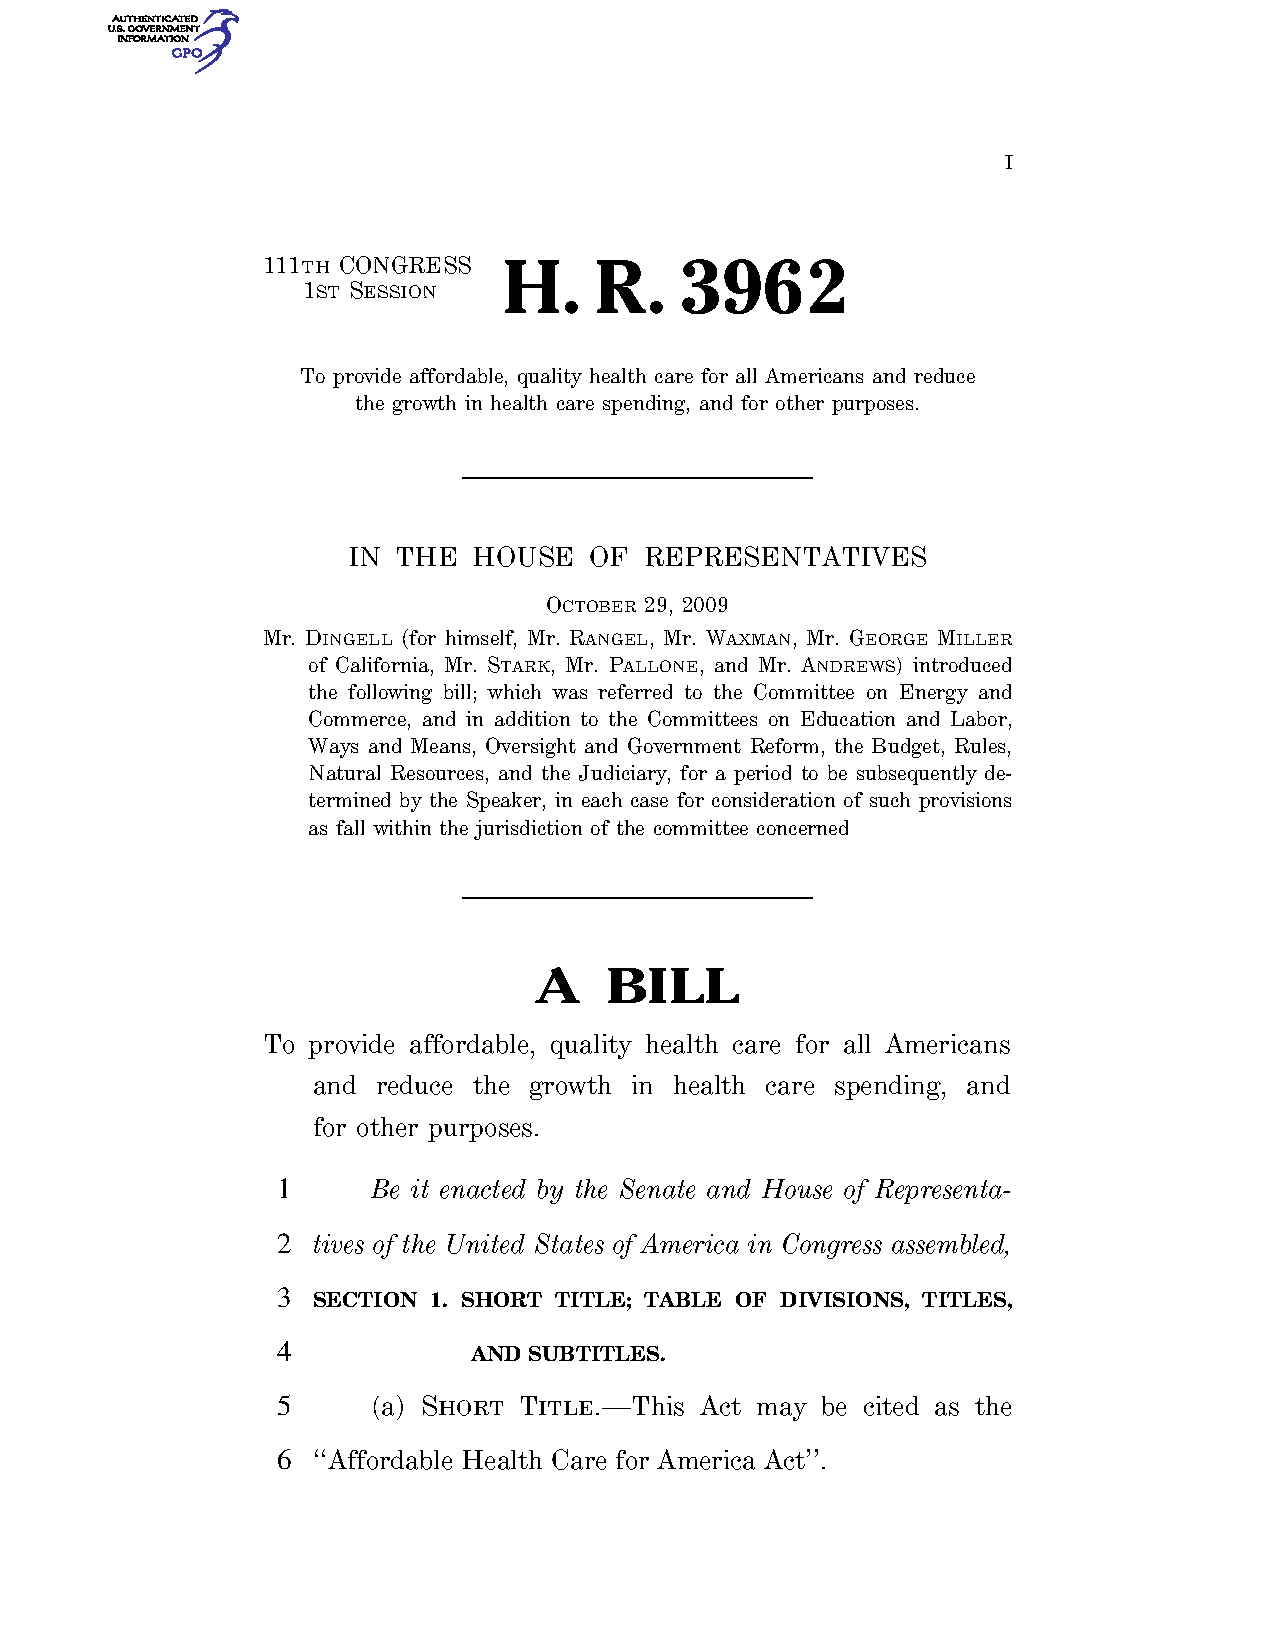
\includegraphics[width=0.3\textwidth]{figs/111_ahcaa-1.pdf}}
    \fbox{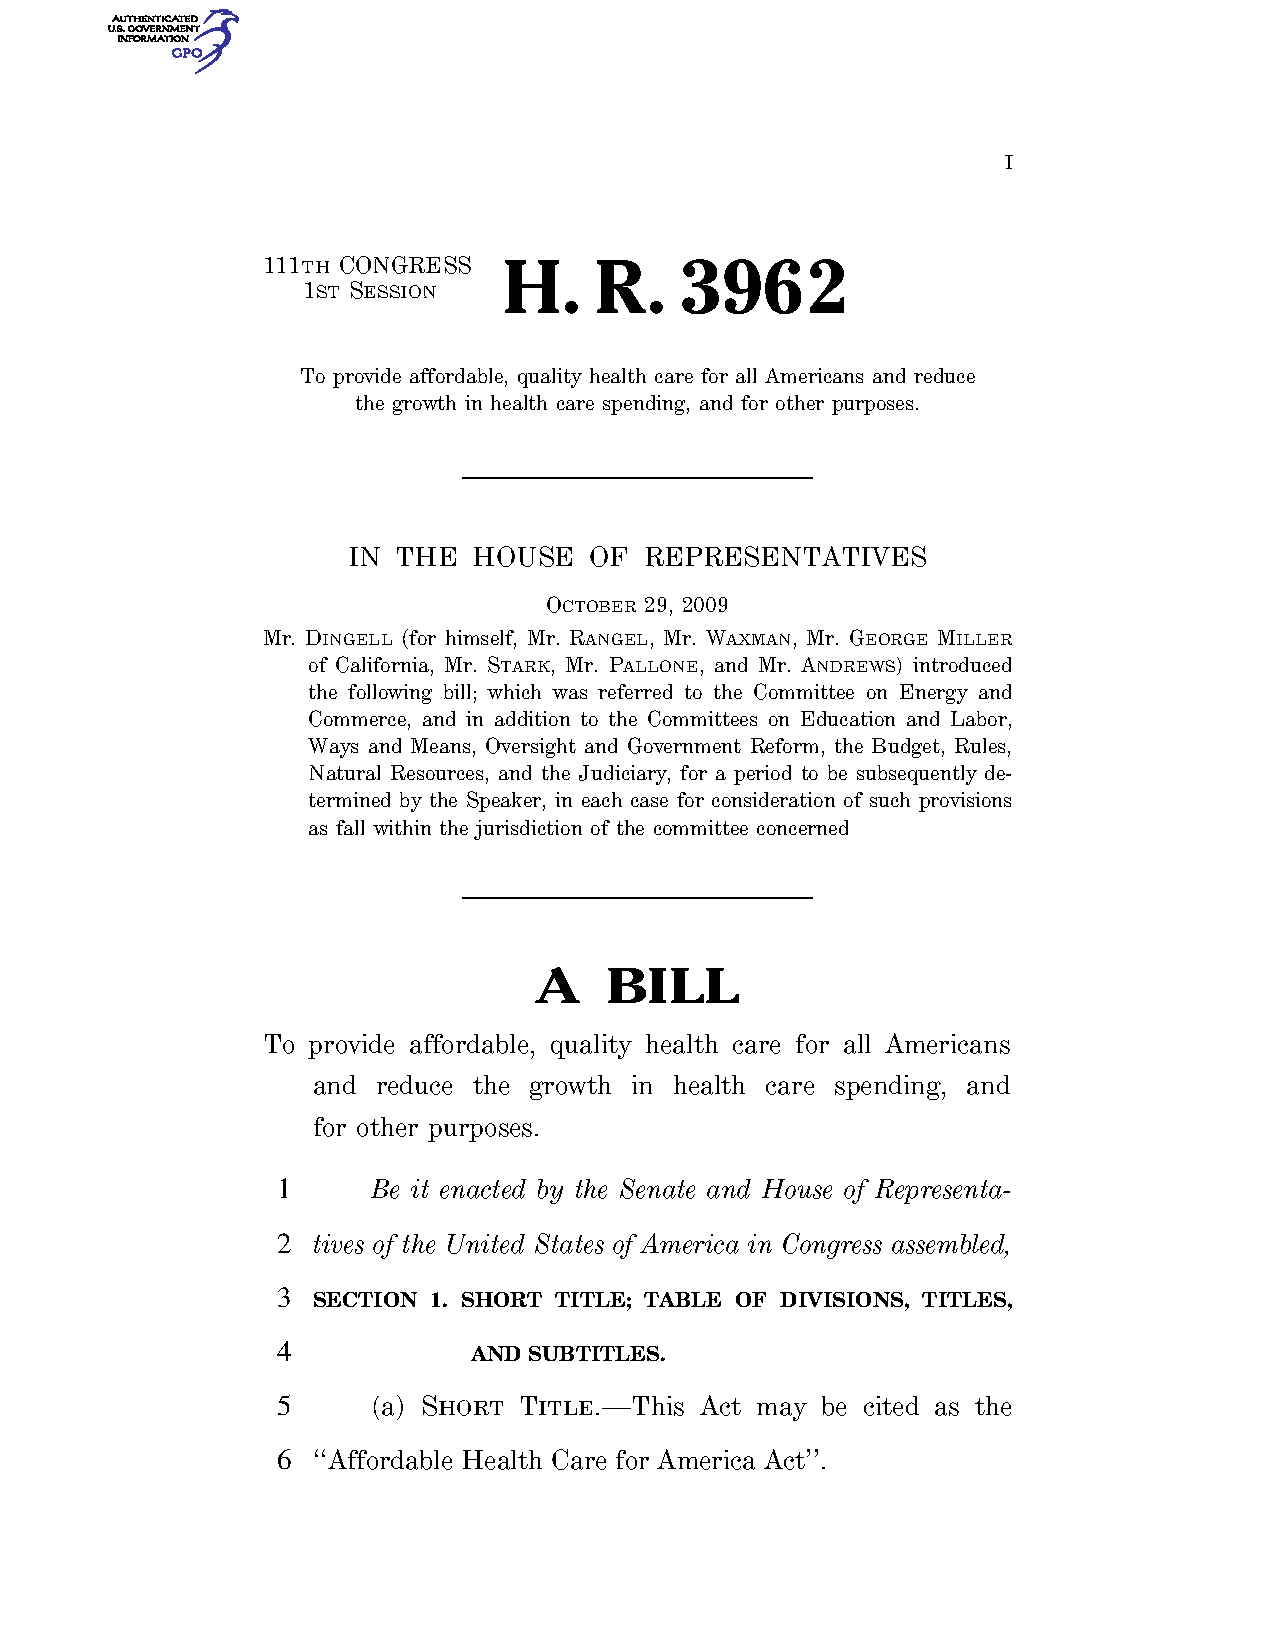
\includegraphics[width=1.0\textwidth]{figs/111_ahcaa-1.pdf}}
    \end{column}
    \begin{column}{0.7\textwidth}
      \begin{itemize}
      \item 276 of 311 Democrats voted ``\textcolor{blue}{Yes}''.
      \item 217 of 217 Republicans voted ``\textcolor{red}{No}''.
        \vspace{20pt}
      \end{itemize}
    \end{column}
  \end{columns}
}

\frame{
  \begin{tabular}{c}
    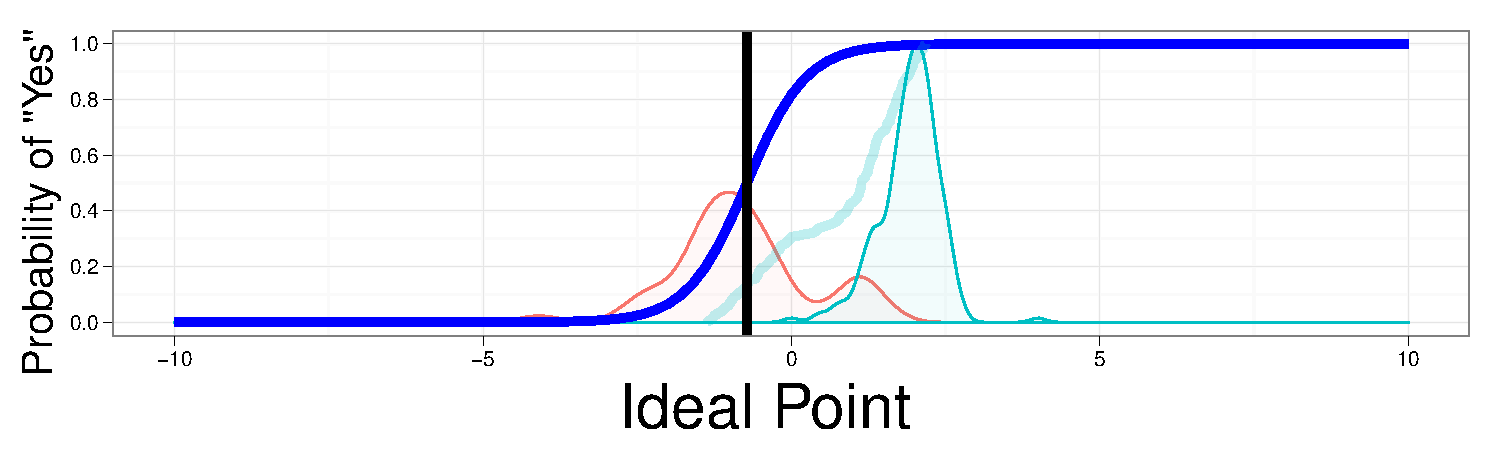
\includegraphics[width=0.8\textwidth]{figs/health_care_logistic.pdf} \\    
  \end{tabular}
  \begin{columns}
    \begin{column}{0.3\textwidth}
%      \setlength\fboxsep{4pt}
%      \setlength\fboxrule{0.5pt}
%    \fbox{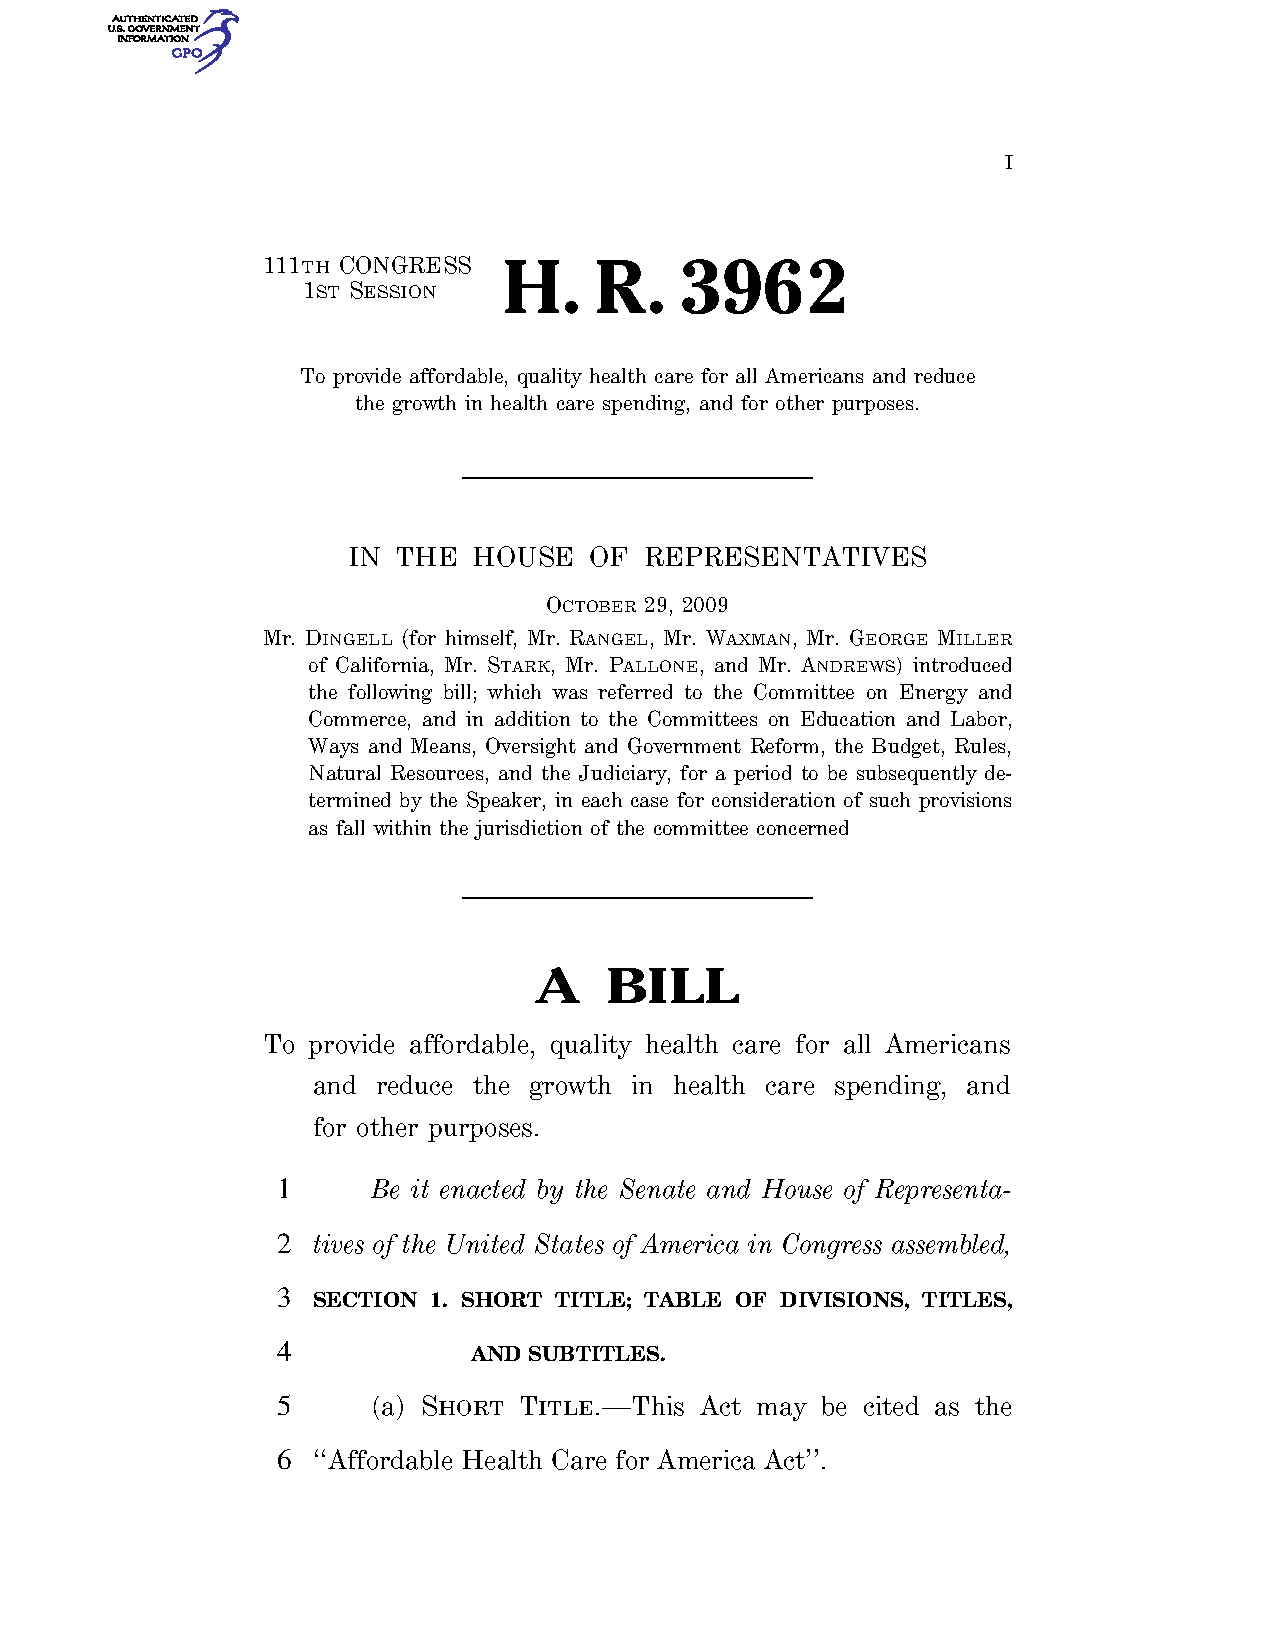
\includegraphics[width=0.3\textwidth]{figs/111_ahcaa-1.pdf}}
    \fbox{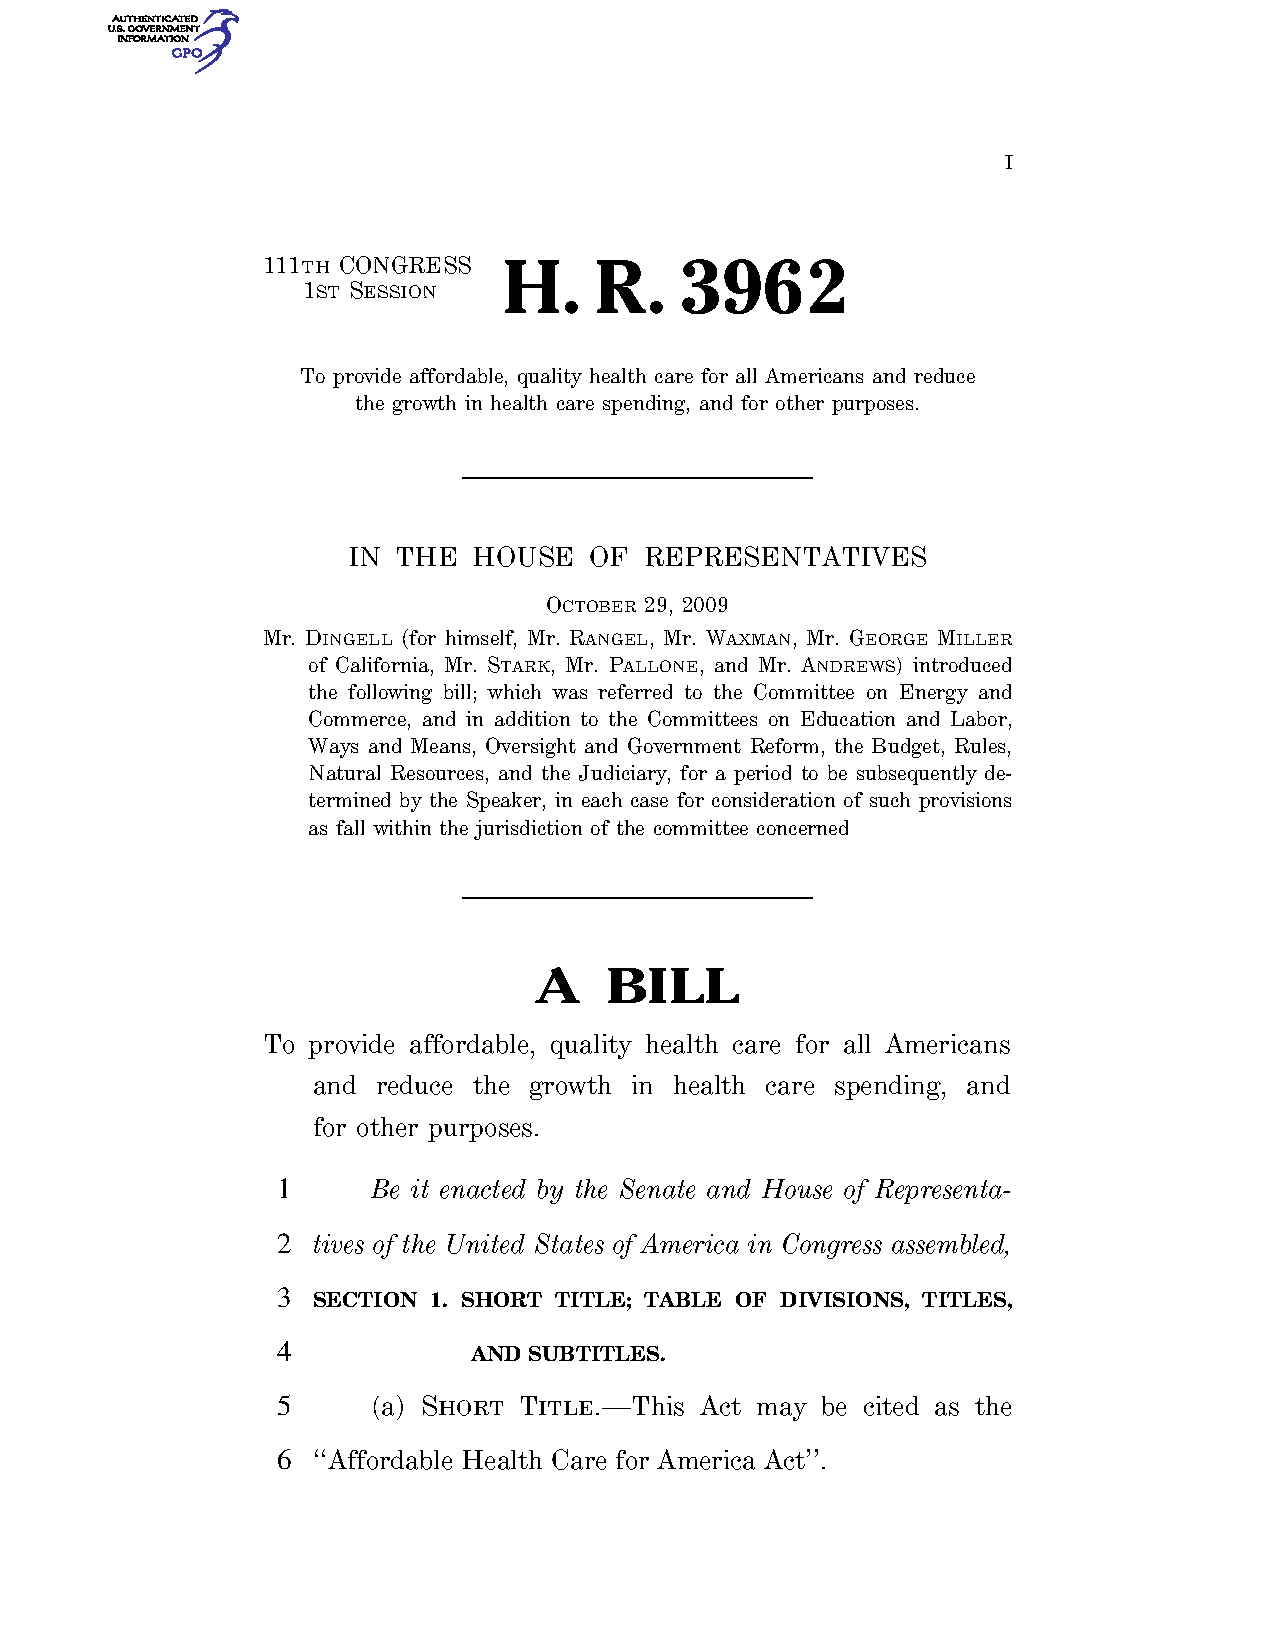
\includegraphics[width=1.0\textwidth]{figs/111_ahcaa-1.pdf}}
    \end{column}
    \begin{column}{0.7\textwidth}
      \begin{itemize}
      \item 276 of 311 Democrats voted ``\textcolor{blue}{Yes}''.
      \item 276 of 276 Republicans voted ``\textcolor{red}{No}''.
      \item Primary topic: \emph{care,applicable,coverage,hospital,eligible}
      \item Inferred bill parameters are \\
        \begin{center} $\lambda_d=1.5$, $\kappa_d=2.1$ \end{center}
      \item Accuracy: 79\%
      \item Baseline accuracy: 51\%
      \end{itemize}
    \end{column}
  \end{columns}
}

\frame{
  \frametitle{Example - Ridge Regression parameters $\eta_{\lambda}, \eta_{\kappa}$}
  \vspace{5pt}
  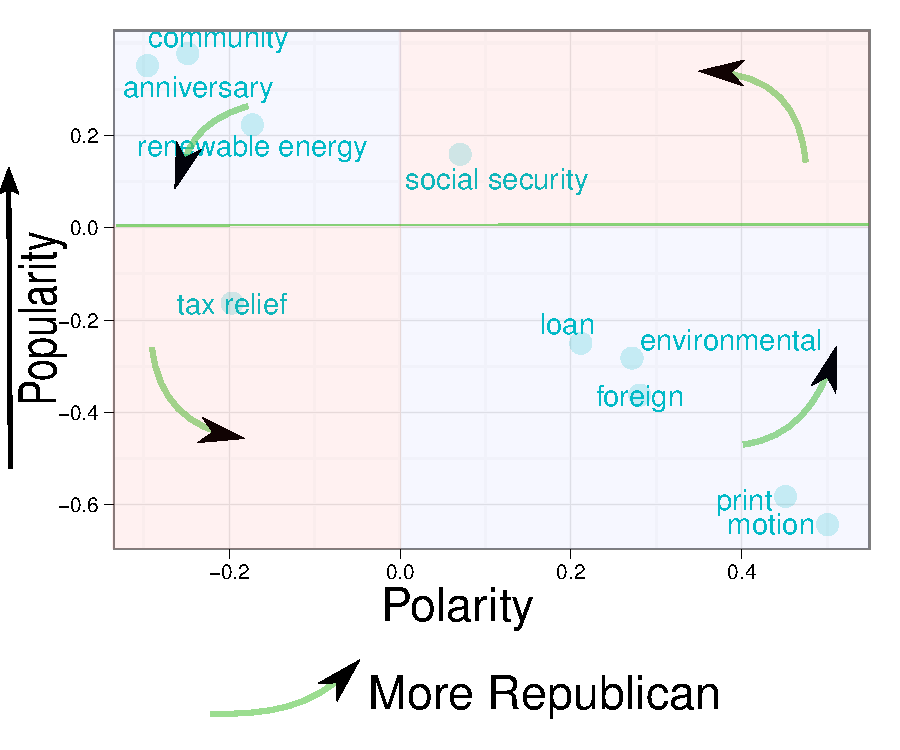
\includegraphics[width=0.9\textwidth]{figs/example_words.pdf}
  With ideal-point text regression, the most popular terms are
  ``life'', ``veterans'', ``hit'', ``federal land'', ``certified'',
  ``post office building'', ``health care'', and ``nationwide''.

  The least-popular terms are ``print'', ``motion offer'', ``tuesday'', ``candidate'', ``whichever'', ``legislative day'', ``prescribe'', and ``bonus''.

  The most right-wing terms are ``life'', ``federal land'', ``veterans'', ``hit'', ``certified'', ``nationwide'', and ``post office building''.
}

\frame{
  \frametitle{Results - Topics}
  \center %\hspace{-30pt}
  \begin{tabular}{|c|l|}
    \hline
    \textbf{Description} & \textbf{Topic summary \tiny (Example words)} \\
    \hline
    Popular & Military recognition
  \tiny (\textcolor{blue}{weteran,war,serve,veterans,training,military}) \normalsize \\
   (high $\bm \eta_{\kappa}$) & Recognition
  \tiny (\textcolor{blue}{people, month, recognize, history, week, woman}) \normalsize \\
  \hline
  Unpopular & \textcolor{gray}{Anything polarizing} \\
  \hline
  Left-wing & Employment and eligibility
  \tiny (\textcolor{blue}{eligible,credit,head,qualified,training}) \normalsize \\  
  (low $\bm -\frac{\eta_{\kappa}}{\eta_{\lambda}}$) & Environmental policy
  \tiny (\textcolor{blue}{energy,emission,epa,administrator,allowance}) \normalsize \\
  & Regulation
  \tiny (\textcolor{blue}{transfer,requires,contract,transportation,expense,corporation}) \normalsize \\
  \hline
  *Right-wing & Social Services
  \tiny (\textcolor{blue}{medicare,social security act,clause,hospital}) \normalsize \\
  (high $\bm -\frac{\eta_{\kappa}}{\eta_{\lambda}}$) & Land management
  \tiny (\textcolor{blue}{land,subtitle,wilderness,river}) \normalsize \\
  & Tobacco
  \tiny (\textcolor{blue}{delivery, cigarette, tobacco, smokeless, sale, bills}) \normalsize \\
  \hline
  \end{tabular}
  %     \end{itemize}
  %   \item Liked by everyone (high $\bm \eta_{\kappa}$): \\
  %     \begin{itemize}
  %       \item Employment and eligibility: \textcolor{blue}{eligible, credit, head, } \\
  %     \end{itemize}
  %   \item Left-wing (low $\bm \eta_{\lambda}$): \\
  %     \begin{itemize}
  %     \item Environmental policy: \textcolor{blue}{energy,emission,epa,administrator,allowance,standard} \\
  %     \item Regulation: \textcolor{blue}{transfer,requires,contract,transportation,expense,corporation}        \\
  %     \item Procedural: \textcolor{blue}{eligible, subparagraph, credit, head, qualified} \\
  %     \end{itemize}
  %   \item Right-wing (high $\bm \eta_{\lambda}$) \\
  %     \begin{itemize}
  %        \item Social Services: \textcolor{blue}{medicare, social security act, clause, hospital} \\
  %        \item Land Management: \textcolor{blue}{land, subtitle, wilderness, river, map, water} \\
  %        \item Tobacco: \textcolor{blue}{delivery, cigarette, tobacco, smokeless, sale, bills} \\
  %     \begin{itemize}
  %   \end{itemize}
}

\frame{
  \frametitle{Results - Topics}
  \center
  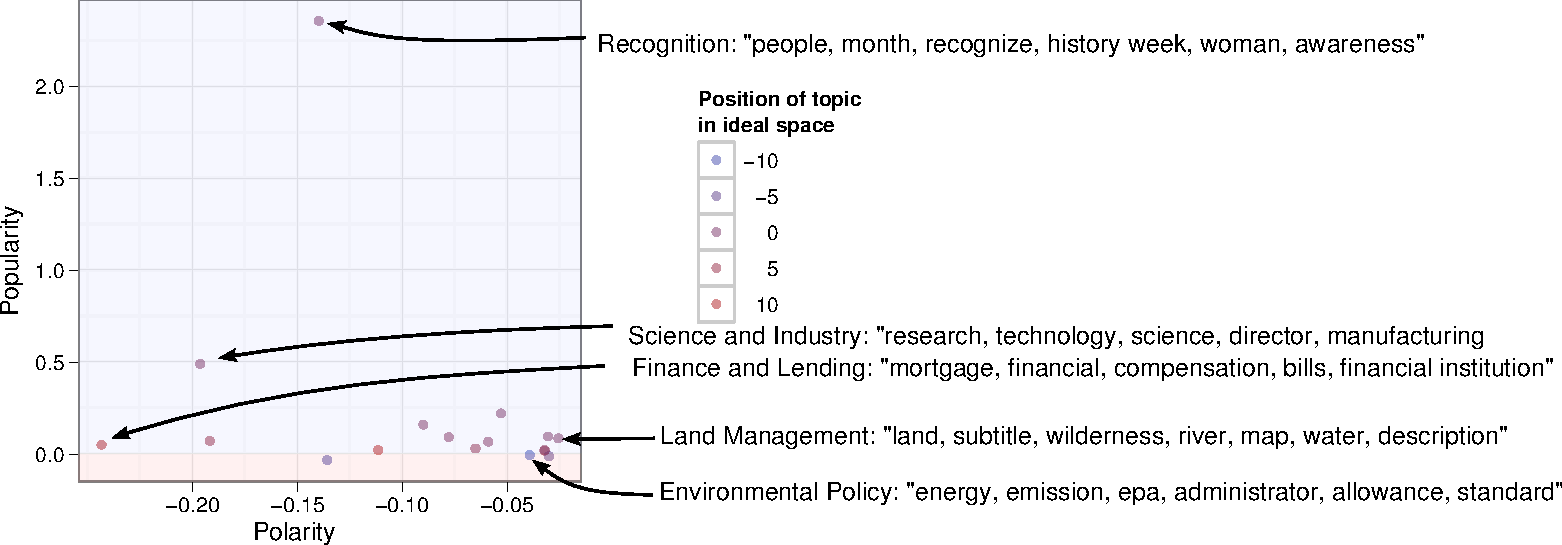
\includegraphics[width=1.0\textwidth]{figs/64_topic_plot.pdf}
}


\frame{
  \frametitle{Results - Prediction}
  \begin{columns}
    \begin{column}{0.5\textwidth}
    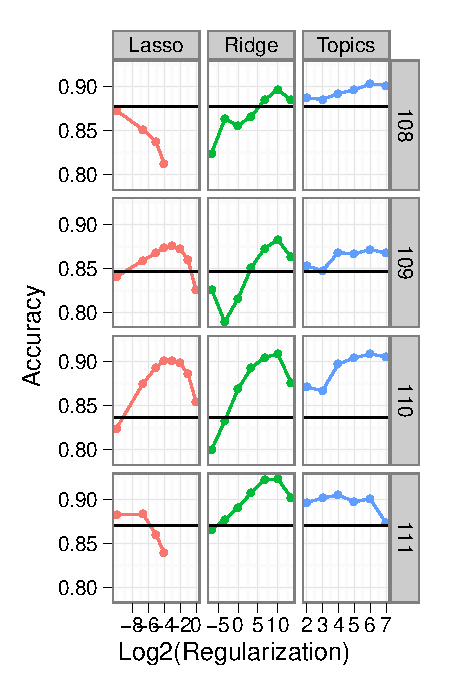
\includegraphics[width=1.0\textwidth]{figs/138_accuracy_by_session_topics_oral.pdf}
%    \includegraphics[width=0.3 \textwidth]{figs/138_log_likelihood_by_session_topics_oral.pdf}
  \end{column}
  \begin{column}{0.5\textwidth}
  \begin{itemize}
    \item Predictive accuracy as high as 92\% with these models
      \vspace{6pt}
    \item Works best for 32-64 topics
      \vspace{6pt}
    \item Baseline ``assume everyone votes yes'' is black horizontal line
    \item 93\% correct votes with a little more effort
  \end{itemize}
  \end{column}
  \end{columns}
}

\frame{
  \frametitle{Current and future directions}
  Model ideal points over time, or with Kalman-type updates \\
  \vspace{12pt}
  Multiple ideal dimensions \\
  \vspace{12pt}
  Apply these models to other datasets: \\
  \begin{itemize}
    \item Content recommendation \\
    \item Keyword-based advertising \\
    \item Music recommendation \\
  \end{itemize}
  \vspace{12pt}
  Use extra information: \\
  \begin{itemize}
    \item Transcripts of floor debates \\
    \item Per-topic ideal points (uses more than 1 dimension) \\
    \item Model ideal points over time \\
  \end{itemize}  
}

\frame{
  \frametitle{Summary}
  The models we have discussed... \\
  \begin{itemize}
    \item Are predictive models for lawmakers' votes, \\
      \vspace{6pt}
    \item Include an exploratory model for discovering politicized topics 
      and understanding the themes driving lawmakers, and \\
      \vspace{6pt}
    \item Have two key ideas at heart, \\
      \vspace{6pt}
      \begin{itemize}
        \item Classic ideal point models \\
            \vspace{6pt}
        \item Supervision with text (e.g., topic models) \\
      \end{itemize}
      \vspace{6pt}
    \item Can be used in a general collaborative filtering setting. \\
  \end{itemize}
}

\frame{
  \frametitle{Contact}
  \begin{center}
    \vspace{-120pt}  
    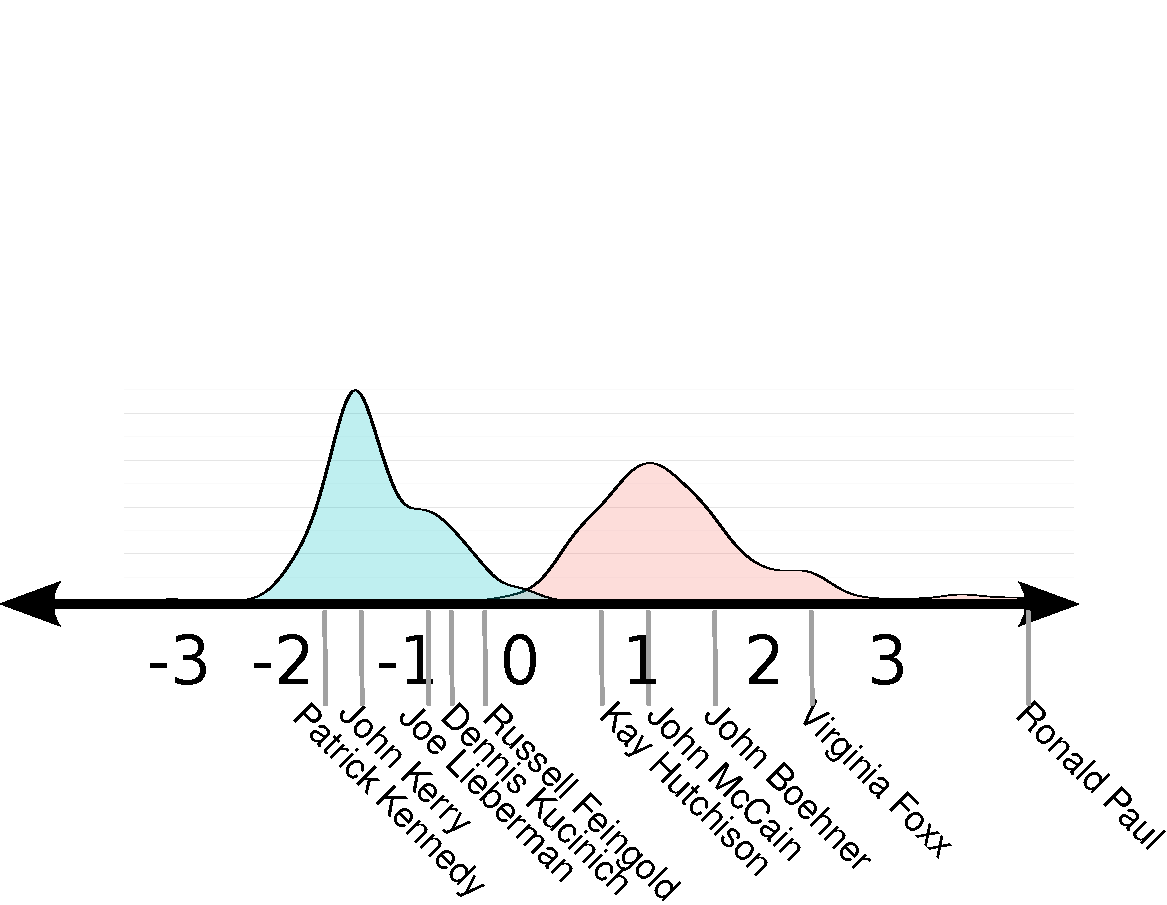
\includegraphics[scale=0.58]{figs/134_interesting_senator_name_accuracy_by_ip_sample_all.pdf}
  \end{center}
  Contact
  \begin{itemize}
    \item Sean Gerrish (sgerrish@cs.princeton.edu)
    \item David Blei (blei@cs.princeton.edu)
  \end{itemize}
  
}


\frame{
  \frametitle{Appendix}
}

\frame{
  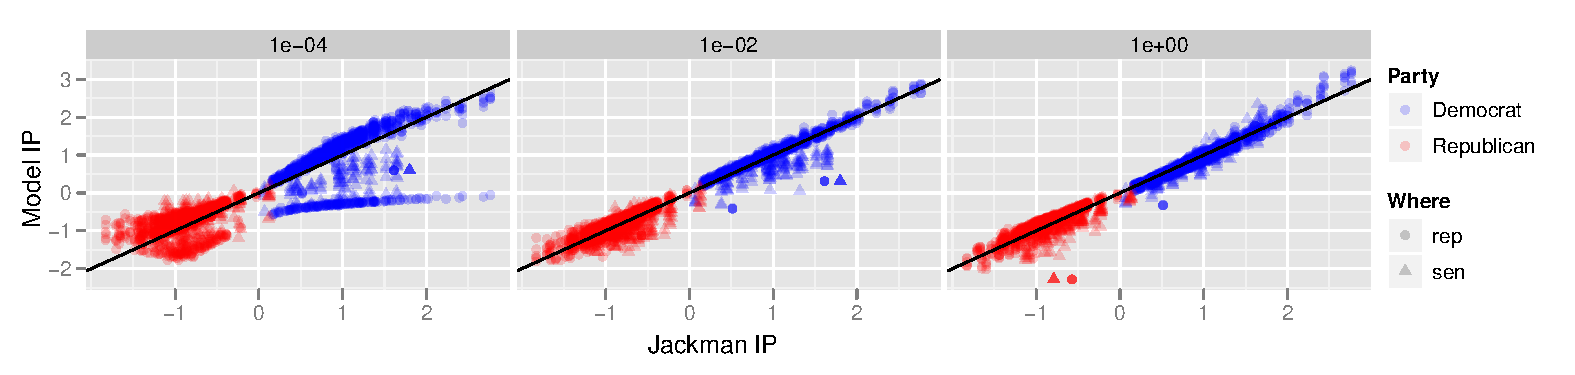
\includegraphics[width=1.0\textwidth]{figs/user_ips_jackman_vs_model_by_dispersion.pdf}
}

\begin{frame}
  \begin{center}
    \LARGE
%    \colorbox{BackgroundBlue}{Ideal point topic models}
    Ideal Point Topic Models
  \end{center}
\end{frame}


\begin{frame}{The ideal point model}
  \begin{center}
    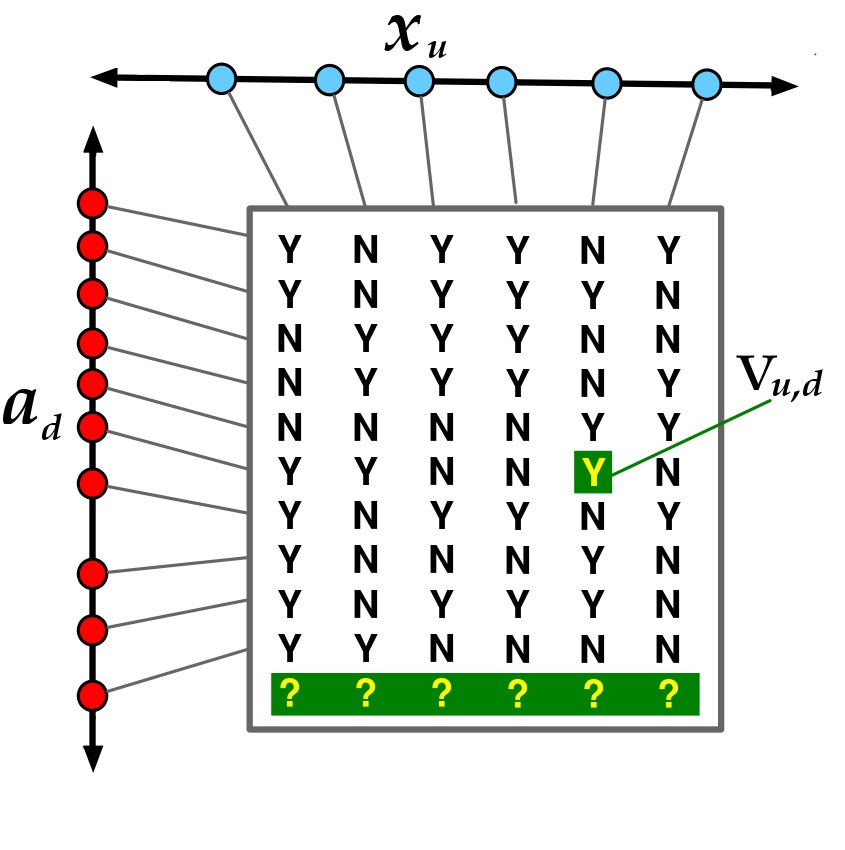
\includegraphics[scale=0.6]{figs/ideal-point-intuition.jpg}
  \end{center}
  \begin{itemize}
  \item A model devised to uncover voting patterns (Clinton et al., 2004).
  \item We observe roll call data $v_{ij}$.
  \item Bills attached to discrimination parameters $a_j$.\\
    Senators attached to ideal points $x_i$.
  \end{itemize}
\end{frame}

%% \begin{frame}{The ideal point model}
%%   \begin{center}
%%     \includegraphics[scale=0.6]{figs/subset-ideal-points.pdf}
%%   \end{center}
%%   \begin{itemize}
%%   \item Posterior inference reveals the political spectrum of senators
%%   \item Widely used in quantitative political science.
%%   \end{itemize}
%% \end{frame}

\begin{frame}{The ideal point model is limited for prediction}
  \begin{center}
    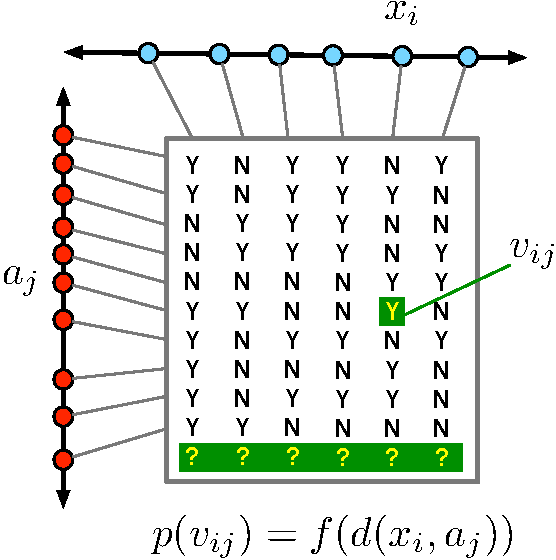
\includegraphics[scale=0.6]{figs/ideal-point-prediction-intuition.pdf}
  \end{center}
  \begin{itemize}
  \item We can predict a missing vote.
  \item But we cannot predict all the missing votes from a bill.
  \item Cf. the limitations of collaborative filtering
  \end{itemize}
\end{frame}

\begin{frame}
  \frametitle{Ideal point topic models}
%  \includegraphics[width=0.85\textwidth]{figs/ideal-point-topic-model-intuition.pdf}
    Use supervised topic modeling assumptions as a predictive
    mechanism from bill texts to bill discrimination.
\end{frame}

\begin{frame}{Ideal point topic models}
  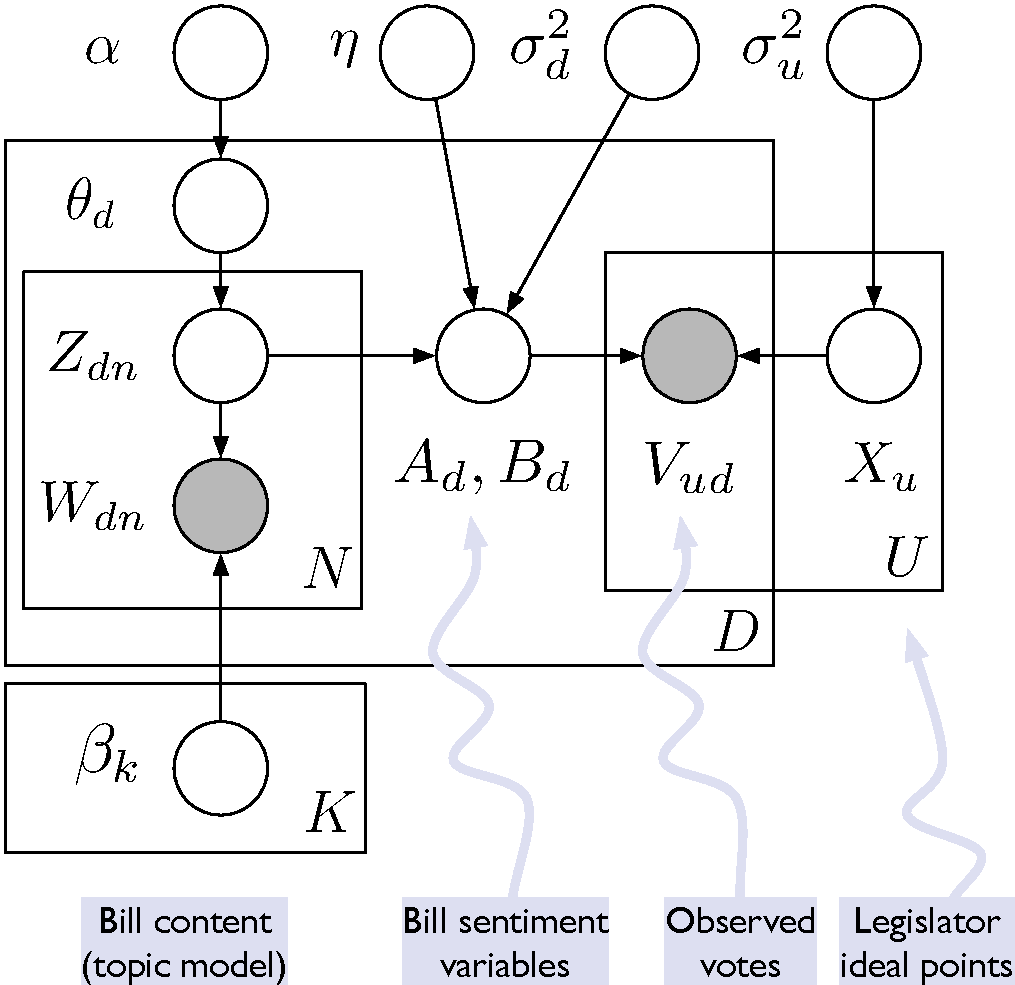
\includegraphics[width=0.45\textwidth]{figs/ideal-point.pdf}
\end{frame}

\begin{frame}{Ideal point topics}
  \includegraphics[width=0.85\textwidth]{figs/ideal-point-topics.pdf}
  In addition to senators and bills, IPTM places \textbf{topics} on the spectrum.
\end{frame}

\begin{frame}{Prediction on completely held-out votes}
  \includegraphics[width=0.75 \textwidth]{figs/vote-accuracy.pdf}
  \begin{center}
    Versus the LASSO, the IPTM correctly predicted 126,000 more
    votes.
  \end{center}
\end{frame}

\begin{frame}{Ideal point topic models}
  \begin{itemize}
  \item Ideal point topic model illustrates
    \begin{itemize}
    \item Topic modeling embedded in a complex model
    \item Topic modeling used to solve a real-world problem with text
    \end{itemize}
  \item More generally, consider collaborative filtering.
    \begin{itemize}
    \item Senators are \textit{users}.
    \item Bills are \textit{items}.
    \end{itemize}
  \item Existing collaborative filtering is akin to classical ideal
    point.
  \item Our model lets us predict preferences on \textit{completely new items}.
  \end{itemize}
\end{frame}

%%% Local Variables: 
%%% mode: latex
%%% TeX-master: "talk"
%%% End: 


\end{document}
